% /*
%  * ----------------------------------------------------------------------------
%  * "THE BEER-WARE LICENSE" (Revision 42):
%  * <michi.wieland@hotmail.com> wrote this file. As long as you retain this notice you
%  * can do whatever you want with this stuff. If we meet some day, and you think
%  * this stuff is worth it, you can buy me a beer in return. Michael Wieland
%  * ----------------------------------------------------------------------------
%  */

\documentclass[
a4paper,
oneside,
10pt,
fleqn,
headsepline,
toc=listofnumbered, 
bibliography=totocnumbered]{scrartcl}

% deutsche Trennmuster etc.
\usepackage[T1]{fontenc}
\usepackage[utf8]{inputenc}
\usepackage[english, ngerman]{babel} % \selectlanguage{english} if  needed
\usepackage{lmodern} % use modern latin fonts

% Custom commands
\newcommand{\AUTHOR}{Michael Wieland}
\newcommand{\INSTITUTE}{Hochschule für Technik Rapperswil}
\newcommand{\GITHUB}{https://github.com/michiwieland/hsr-zusammenfassungen}
\newcommand{\LICENSEURL}{https://en.wikipedia.org/wiki/Beerware}
\newcommand{\LICENSE}{
"THE BEER-WARE LICENSE" (Revision 42):
<michi.wieland@hotmail.com> wrote this file. As long as you retain this notice you
can do whatever you want with this stuff. If we meet some day, and you think
this stuff is worth it, you can buy me a beer in return. Michael Wieland	
}

% Jede Überschrift 1 auf neuer Seite
\let\stdsection\section
\renewcommand\section{\clearpage\stdsection}

% Multiple Authors
\usepackage{authblk}

% Include external pdf
\usepackage{pdfpages}

% Layout / Seitenränder
\usepackage{geometry}

% Inhaltsverzeichnis
\usepackage{makeidx} 
\makeindex

\usepackage{url}
\usepackage[pdfborder={0 0 0}]{hyperref}
\usepackage[all]{hypcap}
\usepackage{hyperxmp} % for license metadata

% Glossar und Abkürzungsverzeichnis
\usepackage[acronym,toc,nopostdot]{glossaries}
\glossarystyle{altlist}
\usepackage{xparse}
\DeclareDocumentCommand{\newdualentry}{ O{} O{} m m m m } {
	\newglossaryentry{gls-#3}{
		name={#4 : #5},
		text={#5\glsadd{#3}},
		description={#6},
		#1
	}
	\makeglossaries
	\newacronym[see={[Siehe:]{gls-#3}},#2]{#3}{#4}{#5\glsadd{gls-#3}}
}
\makeglossaries

% Mathematik
\usepackage{amsmath}
\usepackage{amssymb}
\usepackage{amsfonts}
\usepackage{enumitem}

% Images
\usepackage{graphicx}
\graphicspath{{images/}} % default paths

% Boxes
\usepackage{fancybox}

%Tables
\usepackage{tabu}
\usepackage{booktabs} % toprule, midrule, bottomrule
\usepackage{array} % for matrix tables

% Multi Columns
\usepackage{multicol}

% Header and footer
\usepackage{scrlayer-scrpage}
\setkomafont{pagehead}{\normalfont}
\setkomafont{pagefoot}{\normalfont}
\automark*{section}
\clearpairofpagestyles
\ihead{\headmark}
\ohead{\AUTHOR}
\cfoot{\pagemark}

% Pseudocode
\usepackage{algorithmic}
\usepackage[linesnumbered,ruled]{algorithm2e}

% Code Listings
\usepackage{listings}
\usepackage{color}
\usepackage{beramono}

\definecolor{bluekeywords}{rgb}{0,0,1}
\definecolor{greencomments}{rgb}{0,0.5,0}
\definecolor{redstrings}{rgb}{0.64,0.08,0.08}
\definecolor{xmlcomments}{rgb}{0.5,0.5,0.5}
\definecolor{types}{rgb}{0.17,0.57,0.68}

\lstdefinestyle{visual-studio-style}{
	language=[Sharp]C,
	columns=flexible,
	showstringspaces=false,
	basicstyle=\footnotesize\ttfamily, 
	commentstyle=\color{greencomments},
	morekeywords={partial, var, value, get, set},
	keywordstyle=\bfseries\color{bluekeywords},
	stringstyle=\color{redstrings},
	breaklines=true,
	breakatwhitespace=true,
	tabsize=4,
	numbers=left,
	numberstyle=\tiny\color{black},
	frame=lines,
	showspaces=false,
	showtabs=false,
	escapeinside={£}{£},
}

\definecolor{DarkPurple}{rgb}{0.4, 0.1, 0.4}
\definecolor{DarkCyan}{rgb}{0.0, 0.5, 0.4}
\definecolor{LightLime}{rgb}{0.3, 0.5, 0.4}
\definecolor{Blue}{rgb}{0.0, 0.0, 1.0}

\lstdefinestyle{cevelop-style}{
	language=C++,  
	columns=flexible,
	showstringspaces=false,     
	basicstyle=\footnotesize\ttfamily, 
	keywordstyle=\bfseries\color{DarkPurple},
	commentstyle=\color{LightLime},
	stringstyle=\color{Blue}, 
	escapeinside={£}{£}, % latex scope within code      
	breaklines=true,
	breakatwhitespace=true,
	showspaces=false,
	showtabs=false,
	tabsize=4,
	morekeywords={include,ifndef,define},
	numbers=left,
	numberstyle=\tiny\color{black},
	frame=lines,
}

\lstdefinestyle{eclipse-style}{
	language=Java,  
	columns=flexible,
	showstringspaces=false,     
	basicstyle=\footnotesize\ttfamily, 
	keywordstyle=\bfseries\color{DarkPurple},
	commentstyle=\color{LightLime},
	stringstyle=\color{Blue}, 
	escapeinside={£}{£}, % latex scope within code      
	breaklines=true,
	breakatwhitespace=true,
	showspaces=false,
	showtabs=false,
	tabsize=4,
	morekeywords={length},
	numbers=left,
	numberstyle=\tiny\color{black},
	frame=lines,
}
\lstset{style=eclipse-style}



% Theorems \begin{mytheo}{title}{label}
\usepackage{tcolorbox}
\tcbuselibrary{theorems}
\newtcbtheorem[number within=section]{definiton}{Definition}%
{fonttitle=\bfseries}{def}
\newtcbtheorem[number within=section]{remember}{Merke}%
{fonttitle=\bfseries}{rem}
\newtcbtheorem[number within=section]{hint}{Hinweis}%
{fonttitle=\bfseries}{hnt}

% Dokumentinformationen
\newcommand{\SUBJECT}{Zusammenfassung}
\newcommand{\TITLE}{Mobile and GUI Engineering}

\loadglsentries{glossar}

% pdf metadata
\hypersetup{
	pdfauthor={\AUTHOR},
	pdftitle={\SUBJECT \TITLE},
	pdfcopyright={\LICENSE},
	pdflicenseurl={\LICENSEURL}
}

\begin{document}
	
% Front page
\title{\TITLE}
\subject{\SUBJECT}
\author{\AUTHOR}
\affil{\INSTITUTE}
\date{\today}
\maketitle

\vfill

% Participate
\paragraph{Mitmachen} \hfill \\
Falls Du an diesem Dokument mitarbeiten willst, kannst Du das Dokument
auf GitHub unter \url{\GITHUB} forken.

% Licence
\paragraph{Lizenz} \hfill \\
\LICENSE

% Table of contents
\tableofcontents


% Glossar and acronyms (if included \loadglsentries{glossar})
\printglossary[type=\acronymtype]
\printglossary
\glsaddall


\section{Android}
\subsection{Application}
Die Application Klasse ist der Parent aller Activities. Man kann sich eine eigene Subklasse der Applikation Klasse machen und diese im Manifest.xml angeben
\begin{lstlisting}[caption=Custom Application Class]
<manifest>
	<application android:name="MyApplication">
		<activity></activity>
	</application>	
</manifest>
\end{lstlisting}

\subsection{AndroidManifest.xml}
Das AndroidManifest.xml beinhaltet Beschreibungen, welche global für die App gelten. In ihr sind die Komponenten der App definiert, Metadaten beschrieben, Permissions und Anforderungen and die Geräte API gesetzt. 

\subsection{API Level}
Das API Level definiert welche Versionen von Android unterstützt werden. Aktuell ist API Level 19 (Kitkat) ein recht guter Wert. 
\begin{lstlisting}[caption=API Level Declaration]
<uses-sdk android:minSdkVersion="integer"
	android:targetSdkVersion="integer"
	android:maxSdkVersion="integer" />
\end{lstlisting}

\subsection{APK}
APK ist das Paketformat für Android und grundsätzlich ein \lstinline|JAR| (im Format \lstinline|.zip|), allerdings mit speziellen Class-Dateien.

\subsection{JACK: Java Android Compiler Kit}
Der neue JACK Compiler kompiliert Java Files direkt in Dex Files. Aus den Dex Files wird dann ein APK gebildet.

\subsection{Java 8}
Ab API Level 24 sind folgende Java 8 Features unterstützt
\begin{itemize}
	\item Default und static interface methods (auch verfügbar auf tieferen API Level)
	\item Lamdas
	\item Repeatable annotations
	\item Method Refereces
	\item Type Annotations
\end{itemize}

\section{GUI Komponenten}
Heutzutage befinden wir uns im Post-\gls{wimp} Zeitalter. Es wird jedoch vermehrt auf Fullscreen Applikationen gesetzt.
\begin{description}
	\item[deklartiv] Beschreibung in XML (zu bevorzugen)
	\item[imperativ] in Java Code
\end{description}

\subsection{Klasse R}
Die Klasse R wird vom System automatisch generiert. Sie enthält Konstanten für alle ID's und Ressourcen. Der Zugriff auf die Ressourcen Files erfolgt somit immer über die R Klasse. 

\subsection{Views}
Ist die Basisklasse um ein Interface in Android zu bauen. Alle Views sind hierarchisch strukturiert. Eine View zieht einen rechteckigen Bereich auf, der es erlaubt, Inhalte zu zeichen und Events zu behandeln.

\subsubsection{ViewGroup}
Eine ViewGroup ist eine Unterklasse von View. Sie beinhaltet immer andere Views oder ViewGroups. (Composit Design Pattern) Man spricht auch von Layouts.

\subsubsection{Eigenschaften}
\begin{description}
	\item[ID's] ID's haben immer den Prefix \lstinline|@+id/|. Das Android Buildsystem sammelt dann alle ID's als Konstanten in der Klasse R. \\
	Der Zugriff auf das GUI Objekt erfolgt dann über \lstinline|Button button (Button) findViewById(R.id.myButton)| (Die Methode gibt immer eine View zurück $\rightarrow$ Casten)
	\item[inputType] InputType definiert die Form eines Eingabefeldes. Aufgrund dieser Definition wird eine spezifische Tastatur geladen.
\end{description}

\subsection{Widgets}
Ist ein Sammelbegriff für alle fix-fertigen Komponenten für ein User Interface. 

\subsection{Layouts}
Es können bestehende Layouts verwendet werden, oder auch einen Layouts implementiert werden. Das System generiert automatisch die R-Klasse, welche Konstaten für das Layout enthält. Folgende Layouts werden häufig verwendet:
\begin{description}
	\item[Frame Layout] Mit dem Framelayout können Elemente gestapelt werden. 
	\item[Constraint Layout] ConstraintLayout ist kozeptuell mit dem RelativeLayout verwandt, jedoch optimierter für moderne GUI's.
	\item[WebView Layout] Mit WebView Layout kann HTML angezeigt werden
\end{description}
\begin{figure}[h]
	\centering
	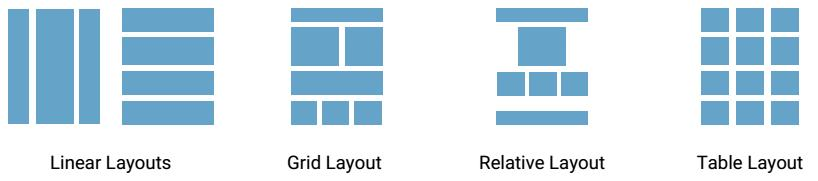
\includegraphics[width=0.7\linewidth]{images/base_layouts}
	\caption{Basis Layouts}
	\label{fig:baselayouts}
\end{figure}

\begin{lstlisting}[caption=Imperatives deklarieren des Layouts]
public class MainActivity extends Activity {
	@Override
	protected void onCreate(Bundle savedInstanceState) {
		super.onCreate(savedInstanceState);
		setContentView(R.layout.activity_main);
	}
}
\end{lstlisting}

\subsubsection{Width und Height}
Alle Views verfügen über die Eigenschaften width und height. Die beiden Eigenschaften erlauben folgende Werte:
\begin{description}
	\item[match\_parent] Nimm den ganzen verfügbaren Platz vom Parent ein
	\item[wrap\_content] Nimm genau den Platz der nötig ist (möglichst klein)
\end{description}

\subsubsection{Linear Layout: Weight}
Im linear Layout definiert das \lstinline|android:layout_weight| wie viel Platz ein Kind gegenüber den anderen Kinder einnimmt.

\subsubsection{Relative Layout}
Beim relativen Layout sind alle Kinder relativ zueinander angeordnet.
\begin{lstlisting}[caption=Relative Layout]
<RelativeLayout xmlns:android="">
	<TextView android:id="@+id/first" />
	<TextView android:id="@+id/first" android:layout_below="@+id/second" /> 
	<TextView android:id="@+id/third" android:layout_toEndOf="@+id/first" /> 
</RelativeLayout>
\end{lstlisting}

\subsection{Ressourcen}
\begin{itemize}
	\item String mit dme @Präfix sind Referenzen auf Ressourcen. 
	\item Ressourcen können sprach-, oder sogar API-abhängig definiert werden.
\end{itemize}

\subsubsection{Strings.xml}
In der Strings.xml können Begriffe ausgelagert, und so einfach übersetzt werden. Der Zugriff erfolgt via \lstinline|getString(R.string.[your key]);|

\begin{lstlisting}[caption=strings.xml,language=xml]
<resources>
	<string name="app_name">My Application</string>
	<string name="hello_world">Hello world!</string>
	<string name="action_settings">Settings</string>
</resources>
\end{lstlisting}

\subsubsection{Dimens.xml}
In \lstinline|Dimens.xml| können Grössenangaben ausgelagert werden. Die definierten Dimensionen können mit \lstinline|@dimen/[dimen name]| geladen werden. Die Angaben sind immer in *.dp rsp. *.dip, welche das Gleiche bedeuten. (\gls{dip}) Bei den Schriften wird \gls{sip} verwendet.
\begin{lstlisting}[caption=dimens.xml, language=xml]
<resources>
<!-- Default screen margins, per the Android Design guidelines. -->
	<dimen name="activity_horizontal_margin">16dp</dimen>
	<dimen name="activity_vertical_margin">16dp</dimen>
</resources>
\end{lstlisting}

\subsubsection{Styles.xml}
Die Styles liegen in \lstinline|res/values/styles.xml|
\begin{lstlisting}[caption=styles.xml, language=xml]
<style name="MyButtonStyle">
	<item name="android:background">#ff85e1</item>
	<item name="android:height">36dp</item>
	<item name="android:minWidth">64dp</item>
	<item name="android:padding">8dp</item>
</style>

<Button
	...
	style="@style/MyButtonStyle"
\end{lstlisting}

\subsection{Events und Listener}
\subsubsection{Event Loop}
Die Event Loop ist eine Endlosschleife, welche auf Ereignise wartet, diese entgegenimmt und sie an die Applikation weiterreicht. Die Event Loop wird oft auch GUI oder Main Thread genannt.

\subsubsection{Event Listener}
Mit Event Listener können auf Events gewartet werden. Eine vollständige Liste aller Events findet man online \footnote{\url{https://developer.android.com/guide/topics/ui/ui-events.html}}. Listener können auch direkt im XML angegeben werden.

\begin{lstlisting}[caption=Event Listener]
button.setOnClickListener(new View.OnClickListener() {
	@Override
	public void onClick(View v) {
	...
	}
});

// fuer mehrere Views
public void onClick(View view) {
	if (view == btn1) {}
	else if (view == btn2) {}
}
\end{lstlisting}


\subsection{Task}
Ein Task ist eine Gruppe von Activities(Abgebildet als Stack). Der Task ist quasi die App, wobei diese auch aus externen Tasks bestehen kann. Man verwendet deshalb unter Android den Begriff des Tasks. Ein Task kann sich über mehrere APKs erstrecken.


\subsection{Context}
Mit der Context Klasse lassen sich:
\begin{itemize}
	\item Neue Views erstellen
	\item auf System Services zugreifen
	\item die Applikationsinstanz erhalten
	\item neue Activities starten
	\item Preferences schreiben und lesen
	\item Services starten
\end{itemize}

\subsection{Activities}
\begin{itemize}
	\item Activity = GUI + Code
	\item Eine Activity ist eine oder mehrere Seiten, die eine Aufgabe oder Aktivität abdecken.
	\item Jede Seite verfügt über GUI Elemente mit Events auf welche reagiert werden kann.
	\item Eine App besteht aus mehreren Activities
	\item Es gibt keine main Methode sondern nur den onCreate() Event der im Parent überschrieben wird
	\item Activities werden in einem Stack organisiert. So popt z.B der Back Button einfach die letzte Activity vom Stack
\end{itemize}

\begin{lstlisting}[caption=Main Activity Grundgerüst]
public class MainActivity extends Activity {
	
	@Override
	protected void onCreate(Bundle savedInstanceState) {
		super.onCreate(savedInstanceState);
		setContentView(R.layout.activity_login);
		
		final EditText emailAddressEditText = (EditText) findViewById(R.id.emailAddressEditText);
		
		findViewById(R.id.loginButton).setOnClickListener(new View.OnClickListener() {
			@Override
			public void onClick(View v) {
				String emailAddress = emailAddressEditText.getText().toString();
				
				// create intent            
				Intent intent = new Intent(CurrentClass.this, TargetClass.class);
				
				// pass param to new intent
				intent.putExtra(Intent.EXTRA_EMAIL, emailAddress);
				
				// open new activity
				startActivity(intent);
			}
		});
	}
}
\end{lstlisting}


\subsubsection{Lifecylce}
Die einzelnen Event-Methoden können in der Activity Klasse überschrieben werden.

\begin{figure}[h]
\centering
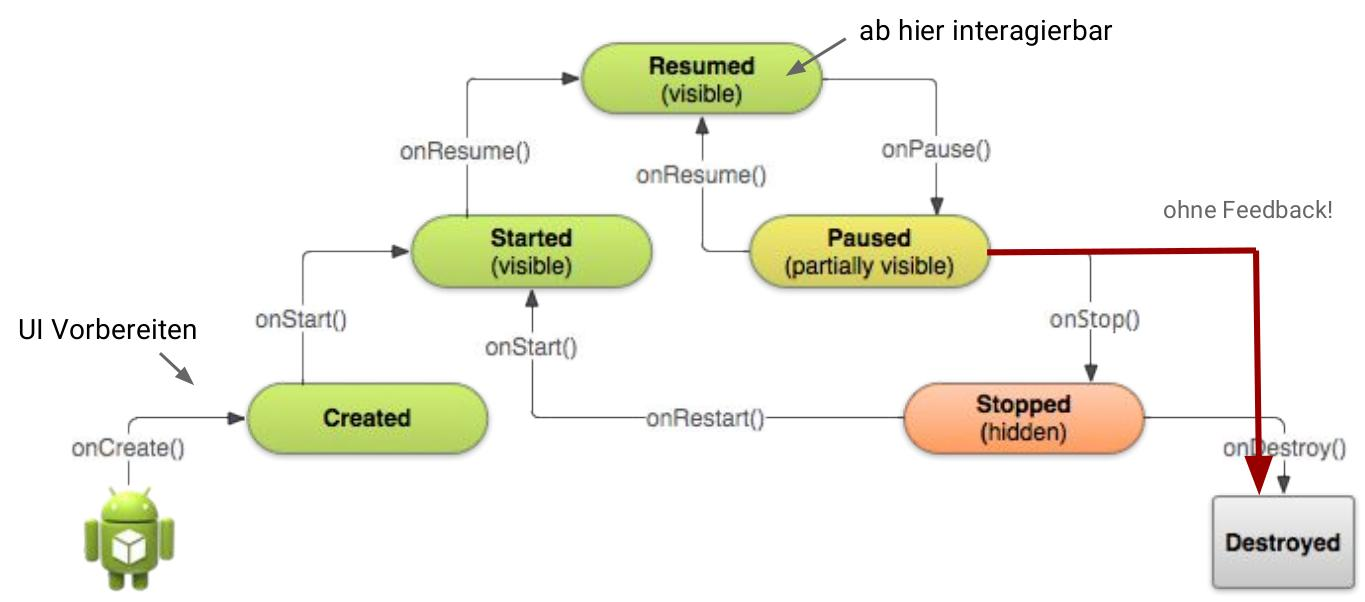
\includegraphics[width=0.7\linewidth]{images/android_lifecycle}
\caption{Activity Lebsnzyklus}
\label{fig:androidlifecycle}
\end{figure}

\begin{remember}{Daten persistent speichern}{}
Daten in onPause sichern, da wir nicht darauf vertrauen können, dass onStop oder onDestroy aufgerufen werden!
\end{remember}

\begin{description}
	\item[Starten der App] onCreate() -> onStart() -> onResume()
	\item[Sperren des Screens] onPause() -> onStop()
	\item[Entsperren des Screens] onRestart() -> onStart() -> onResume()
	\item[Beenden mit dem Backbutton] onDestroy()
\end{description}


\paragraph{Paused / Resumed}
\begin{itemize}
	\item Wird die Activity von einer anderen Activity überdeckt, wird erstere pausiert
	\item Kommt sie dann wieder in den Vordergrund, wird wieder onResume aufgerufen
\end{itemize}

\paragraph{Stopped / Started}
\begin{itemize}
	\item Kommt die Activity wieder in den Vorderund, z.B. weil der User die Applikation
	nochmal startet oder mit dem Back-Button zurückkommt, dann wird onRestart
	aufgerufen
\end{itemize}

\paragraph{Destroyed}
\begin{itemize}
	\item Destroyed wird die App vom System oder wenn explizit vom User geschlossen
	\item Dies kann auch direkt aus dem Paused-Zustand geschehen!
	\item Activity wird z.B. bei Änderung der Screen-Orientierung destroyed.
\end{itemize}


\subsubsection{Launch Modes}
Launch Modes beschreiben wie eine neue Instanz einer Aktivität mit dem aktuellen Task assoziiert wird.
\begin{description}
	\item[Standard] Die neue Aktivität wird dem bestehenden Task hinzugefügt
	\item[singleTop] Wenn die neue Aktivität bereits im bestehenden Task existiert wird die neue Aktivät auf die bestehende gemapt.
	\item[singleTask] Für die neue Aktivität wird ein neuer Task erstellt (Browser, Maps)
	\item[singleInstance] Gleich wie singleTask mit dem Unterschied das ein Task nur eine einzelne Aktivität beinhaltet und für alle weiteren neuen Aktivitäten wieder einen neuen Task erstellt.
\end{description}

\subsection{Fragments}
Ein Framgment ist ein modularer Teil der Activity, mit eigenem Lifecycle. Ein Fragment kann in unterschiedlichen Activites eingebunden werden, weshalb sie keine Abhängigkeiten zur Activity haben dürfen. Fragments sind eine gute Möglichkeit, um Wiederverwendbare Komponente zu erstellen. 

\paragraph{Fragment oder Activity?}
\begin{itemize}
	\item Braucht man einen möglichen Eintrittspunk $\rightarrow$ Activity
	\item Ansonsten $\rightarrow$ Fragment
\end{itemize}

\begin{lstlisting}[caption=Fragment]
public class MainActivityFragment extends Fragment implements View.OnClickListener {

	public interface OnItemSelectedListener {
		void onItemSelected(String item);
	}

	@Override
	public void onAttach(Context activity) {
		super.onAttach(activity);
		if (!(activity instanceof OnItemSelectedListener)) {
			throw new AssertionError("Activity must implement View.OnClickListener!");
		}
	}
		
	@Override
	public View onCreateView(LayoutInflater inflater, ViewGroup container, Bundle savedInstanceState) {
		// false bedeutet, dass die View nicht in den Container eingefuegt werden soll, da das bereits das Fragment macht
		View root = inflater.inflate(R.layout.my_fragment, container, false);
		
		Button nextButton = (Button) root.findViewById(R.id.nextButton)
		nextButton.setOnClickListener((View.OnClickListener) getActivity());
		
		return root;
	}	
	
	@Override
	public void onClick(View v) {
		OnItemSelectedListener parentActivity = (OnNewsletterSubscription) getActivity();
		parentActivity.onItemSelected("Test");
	}
}
\end{lstlisting}

\subsubsection{Lifecycle}
Fragments haben gegenüber der Activity zusätzliche Zustände
\begin{itemize}
	\item onAttach(): Fragement wird einer Activity hinzugefügt
	\item onDetach(): 
	\item onCreateView(): UI des Fragment erstellen
	\item onActivityCreated(): wenn Activity onCreate() abgeschlossen ist
	\item onDestroyView(): Gegenstück zum onCreateView();
\end{itemize}

\subsubsection{Kommunikation}
Das Fragment definiert ein Interface zur Kommunikation, welches die Parent Activity implementieren muss.

\subsubsection{Einbinden}
Fragment können auf zwei Möglichkeiten eingebunden werden
\begin{itemize}
	\item statisch
	\item dynamisch (Fragments lassen sich austauschen)
\end{itemize}

\begin{lstlisting}[caption=Statisches Einbinden eines Fragment in XML, language=XML]
<LinearLayout ...>
   <fragment
	   android:id="@+id/fragment"
	   android:name="com.example.myfragmentapplication.MainActivityFragment"
	   android:layout_width="match_parent"
	   android:layout_height="match_parent"
	   tools:layout="@layout/fragment_main" />
</LinearLayout>
\end{lstlisting}
\begin{lstlisting}[caption=Statisches Einbinden eines Fragment im Code]
public class MainActivity extends AppCompatActivity {
	@Override
	protected void onCreate(Bundle savedInstanceState) {
		super.onCreate(savedInstanceState);
		setContentView(R.layout.activity_main);
	}
}
\end{lstlisting}

\begin{lstlisting}[caption=Dynamisches Einbinden eines Fragment in XML, language=XML]
<?xml version="1.0" encoding="utf-8"?>
<RelativeLayout xmlns:android="http://schemas.android.com/apk/res/android"
	android:id="@+id/fragment_container"
	android:layout_width="match_parent"
	android:layout_height="match_parent" />
\end{lstlisting}


\begin{lstlisting}[caption=Dynamisches Einbinden eines Fragment im Code]
public class MainActivity extends Activity {
	@Override
	protected void onCreate(Bundle savedInstanceState) {
		super.onCreate(savedInstanceState);
		setContentView(R.layout.activity_main);
	
		FragmentManager fragmentManager = getFragmentManager();
		FragmentTransaction fragmentTransaction = fragmentManager.beginTransaction();
	
		MainActivityFragment fragment = new MainActivityFragment();
		fragmentTransaction.add(R.id.fragment_container, fragment);
		fragmentTransaction.commit();
	}
}
\end{lstlisting}


\subsection{Intents}
Mit Intents können Daten zwischen zwei Activities ausgetauscht werden. Man unterscheidet zwischen expliziten Intents, bei der Daten direkt von einer bestimmten Komponente abgefragt werden und impliziten Intents, bei dem im Android System nach Komponenten (Handlern) gesucht wird, welche die gesuchten Daten zur Verfügung stellen können. Intent werden immer an das System propagiert, welches dann entscheidet wer dafür zuständig ist.

Mit Intents können Parameter mitgegeben werden (z.B. eine Link-URL für den Browser). Übergeben werden können nur Primitive Daten, Strings sowie alle \emph{serialisierbaren} Objekte.

\begin{lstlisting}[caption=Expliziter Intent mit der Klasse]
new Intent(CurrentClass.this, CalculateActivity.class)
\end{lstlisting}
\begin{lstlisting}[caption=Impliziter Intent mit einer Aktion]
new Intent(MediaStore.ACTION_IMAGE_CAPTURE)
\end{lstlisting}


\begin{lstlisting}[caption=Intents]
startActivityForResult(intent, SOME_ID);

@Override
protected void onActivityResult(int request, int result, Intent data) {
	if (result == Activity.RESULT_OK && request == SOME_ID) {
		// Resultat verarbeiten
	}
}
\end{lstlisting}



\subsection{Broadcast Receiver}
Broadcast Receiver können registriert werden, um auf System Ereignisse oder von anderen Apps zu hören. Broadcasts sind Intents, die versendet werden. Der Receiver sollte im onResume() registriert werden und im onPause() wieder abgemolden werden.
\begin{lstlisting}[caption=Broadcast Receiver]
LocalBroadcastManager lbm = 
LocalBroadcastManager.getInstance(getApplicationContext());
IntentFilter filter = new IntentFilter(Intent.ACTION_BOOT_COMPLETED);
MyBroadcastReceiver receiver = new MyBroadcastReceiver(this);
lbm.registerReceiver(receiver, filter);
\end{lstlisting}


\subsection{Content Provider}
Ein Content Provider stellt Daten prozessübergreifen zur Verfügung. Provider und Consumer kommunizieren über eine standardisierte Schnittstelle um Daten auszutauschen (Client-Server Modell). Android selbst stellt Daten (Kalender, Kontakte) mit einem Content Provider zur verfügung.
\begin{lstlisting}[caption=Content Provider Client]
Cursor cursor = getContentResolver().query(
	UserDictionary.Words.CONTENT_URI,
	mProjection,
	mSelectionClause,
	mSelectionArgs,
	mSortOrder);
	
int index = cursor.getColumnIndex(UserDictionary.Words.WORD);
while (cursor.moveToNext()) {
	String word = cursor.getString(index);
}
\end{lstlisting}

\subsection{TextWatcher}
Textwatcher werden für die Inputvalidierung eingesetzt. Meistens wird dabei \lstinline|onTextChanged| eingesetzt, möglich wäre aber auch \lstinline|beforeTextChanged| und \lstinline|afterTextChanged|
\begin{lstlisting}[caption=TextWatcher]
final EditText password = (EditText) findViewById(R.id.password);
password.addTextChangedListener(new TextWatcher() {

	@Override
	public void afterTextChanged(Editable s) {
		String pw = s.toString();
		if (s.length() < 8) {
			password.setError("Passwort muss mindestens 8 Zeichen lang sein.");
		}
	}
...
});
\end{lstlisting}


\section{GUI Design}
\subsection{Ablauf}
Beim erstellen einer App ist folgender Ablauf empfehlenswert
\begin{enumerate}
	\item Domain Modell erstellen
	\item Screen Map ableiten
	\begin{itemize}
		\item Screens gruppieren (z.B für den Einsatz auf dem Tablet)
	\end{itemize}
	\item Beziehungen der Screens definieren und gruppieren
	\begin{itemize}
		\item Parent Child (Descendant Navigation)
		\item Siblings (Lateral Navigation)
	\end{itemize}
	\item Navigation ableiten
	\begin{itemize}
		\item Ancestral Navigation: zurück zum hierarchischen Parent (Up und Home Button)
		\item Temporal Navigation: zurück zum vorherigen Element (Back Button)
	\end{itemize}
	\item Wireframe/Storyboard für die Gesamtübersicht erstellen
	\item Usability Tests mit einem Paper Prototypen des Wireframe erstellen
\end{enumerate}

\begin{figure}[ht!]
	\centering
	\begin{minipage}[t]{0.4\textwidth}
		\centering
		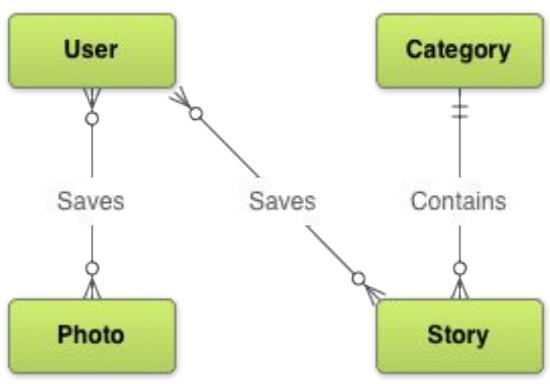
\includegraphics[width=0.7\linewidth]{images/domain_model}
		\caption{Domain Modell}
		\label{fig:domainmodel}
	\end{minipage}
	\begin{minipage}[t]{0.4\textwidth}
		\centering
		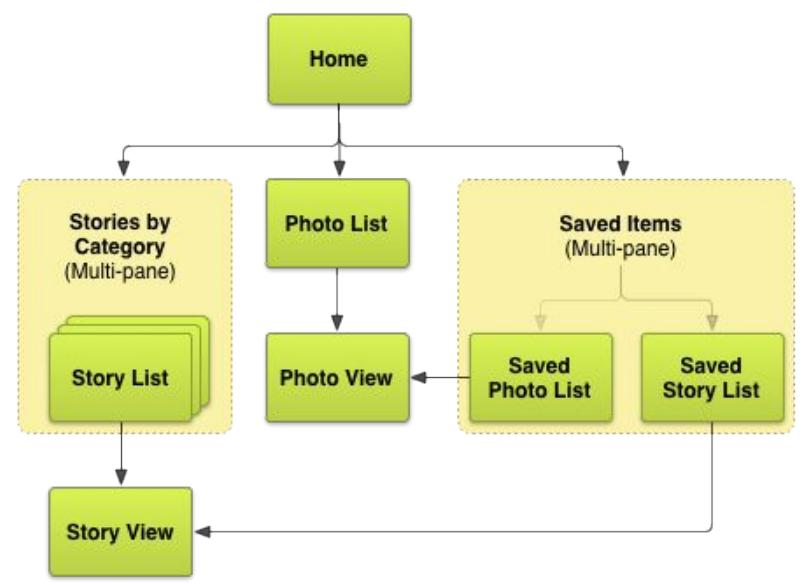
\includegraphics[width=0.7\linewidth]{images/screenmap}
		\caption{Screenmap mit Gruppen}
		\label{fig:screenmap}
	\end{minipage}
\end{figure}

\subsection{Master Detail View}
Damit zwischen Mobiltelefon und Tablet unterschieden werden kann, überprüft man ein Fragment vorhanden ist.
\begin{lstlisting}[caption=Master Detail View]
public class ItemListActivity extends Activity implements ItemListFragment.Callbacks {
	private boolean twoPane;

	@Override
	protected void onCreate(Bundle savedInstanceState) {
		super.onCreate(savedInstanceState);
		setContentView(R.layout.activity_item_list);
		if (findViewById(R.id.item_detail_container) != null) {
			twoPane = true;
		}
	}
	
	 @Override
	 public void onItemSelected(String id) {
		 if (twoPane) {
			 Bundle arguments = new Bundle();
			 arguments.putString(ItemDetailFragment.ARG_ITEM_ID, id);
			 ItemDetailFragment fragment = new ItemDetailFragment();
			 fragment.setArguments(arguments);
			 getFragmentManager()
				 .beginTransaction()
				 .replace(R.id.item_detail_container, fragment)
				 .commit();
		 } else {
			 Intent detailIntent = new Intent(this, ItemDetailActivity.class);
			 detailIntent.putExtra(ItemDetailFragment.ARG_ITEM_ID, id);
			 startActivity(detailIntent);
		 }
	 }
}
\end{lstlisting}


\section{Widgets}
\subsection{Menüs}
%TODO Settings Page
\begin{itemize}
	\item Auch Fragmente können Einträge in dem Menü der Activity einfügen
\end{itemize}
\begin{lstlisting}[caption=Menue in XML, language=XML]
<menu xmlns:android="http://schemas.android.com/apk/res/android"
xmlns:tools="http://schemas.android.com/tools" tools:context=".MainActivity">
	<item android:id="@+id/action_search" 
		android:title="@string/action_search"
		android:icon="@drawable/ic_action_search"
		android:orderInCategory="100"
		android:showAsAction="never" />

	<item android:id="@+id/action_settings"    
		android:title="@string/action_settings"
		android:orderInCategory="100"
		android:showAsAction="never" />
</menu>
\end{lstlisting}

\begin{lstlisting}[caption=Menue]
public boolean onCreateOptionsMenu(Menu menu) {
	// Inflate the menu; this adds items to the action bar if it is present.
	getMenuInflater().inflate(R.menu.menu_main, menu);
		return true;
	}
	public boolean onOptionsItemSelected(MenuItem item) {
		switch (item.getItemId()) {
			case R.id.action_search:
			// handle start
			return true;
			...
}
\end{lstlisting}

\subsection{Toolbars}
\begin{lstlisting}[caption=Toolbar in XML, language=XML]
<RelativeLayout xmlns:android="..." xmlns:app="..." xmlns:tools="..."
android:layout_width="match_parent" android:layout_height="match_parent"
tools:context=".MainActivity">
	<android.support.v7.widget.Toolbar
		android:id="@+id/toolbar"
		android:layout_width="match_parent"
		android:layout_height="wrap_content">
	</android.support.v7.widget.Toolbar>

	<fragment 
		...
		android:layout_below="@+id/toolbar"
		tools:layout="@layout/fragment_main" />
</RelativeLayout>
\end{lstlisting}

\begin{lstlisting}[caption=Toolbar verwenden]
public class MainActivity extends AppCompatActivity {
	@Override
	protected void onCreate(Bundle savedInstanceState) {
		super.onCreate(savedInstanceState);
		setContentView(R.layout.activity_main);
		Toolbar toolbar = (Toolbar) findViewById(R.id.toolbar);
		setSupportActionBar(toolbar);
	}
}
\end{lstlisting}

\subsection{Navigation Drawer}
\begin{itemize}
	\item Der Navigation Drawer kann als Hauptmenü verwendet werden
	\item Das Problem ist aber, dass die Optionen nicht mehr gefunden werden.
	\item Falls man den Navigation Drawer verwenden möchte, sollte es genügend Hinweise auf das Menü geben.
	\item Benötigt eine Support Library
\end{itemize}

\subsection{Snackbar}
Snackbar löst den Toast für Feedback-Nachrichten ab

\subsection{ListView}
Im Adapter Pattern ist die List View der Client.
\begin{lstlisting}[caption=List View XML Declaration, language=XML]
<ListView
   android:layout_width="match_parent"
   android:layout_height="match_parent"
   android:id="@+id/listView"/>
\end{lstlisting}

\begin{lstlisting}[caption=List View mit AdapterView]
ArrayAdapter<String> adapter = new ArrayAdapter<String>(this, android.R.layout.simple_list_item_1, yStringArray);
listView.setAdapter(adapter);
\end{lstlisting}

\begin{figure}[h]
\centering
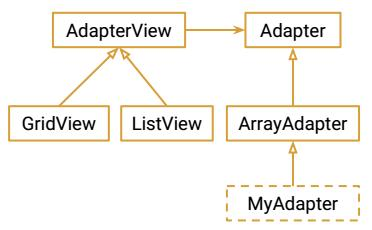
\includegraphics[width=0.4\linewidth]{images/adapter_view}
\caption{Adapter View Klassenmodell}
\label{fig:adapterview}
\end{figure}

\subsubsection{View Tags}
Damit eine View nicht immer wieder erstellt wird, kann sie getagt werden.
\begin{lstlisting}[caption=ViewTag]
public View getView(int position, View convertView, ViewGroup parent) {

if (convertView == null) {
...

TextView textView = (TextView) convertView.findViewById(R.id.textView);
CheckBox checkBox = (CheckBox) convertView.findViewById(R.id.checkBox);

// Pair is the view holder
Pair<TextView, CheckBox> views = new Pair<>(textView, checkBox);
convertView.setTag(views);
}

Pair<TextView, CheckBox> views = (Pair<TextView, CheckBox>) convertView.getTag();
TextView textView = views.first;
CheckBox checkBox = views.second;
}
\end{lstlisting}


\subsection{Recycle View}
Die Recylce View ist der Nachfolger der List und GridView. Im Gegensatz zu seinen Vorgänger bietet sie standardmässig ein Recycling von Elementen und mehrerere Layoutmanager sowie Animationen. Der Nachteil ist das mühsamere Click-Handling.
\begin{lstlisting}[caption=Recycler View]
public class MyAdapter extends RecyclerView.Adapter<ViewHolder> {
	private ArrayList<Module> dataset;
	public MyAdapter(ArrayList<Module> modules) { dataset = modules; }
	public ViewHolder onCreateViewHolder(ViewGroup parent, int viewType) { ... }
	public void onBindViewHolder(ViewHolder holder, int position) { ... }
	public int getItemCount() {
		return dataset.size();
	}
	
	recyclerView = (RecyclerView) rootView.findViewById(R.id.recyclerView);
	layoutManager = new LinearLayoutManager(getActivity());
	recyclerView.setLayoutManager(layoutManager);
	adapter = new ...
	recyclerView.setAdapter(adapter);
}
\end{lstlisting}

\subsection{Card View}
Card View erbt vom Frame Layout und rendert den Content innerhalb von sogenannten Karten. Man kann die Karten mit Schatten und Runde Ecken darstellen.
\begin{lstlisting}[caption=Card View]
<LinearLayout xmlns:android="http://schemas.android.com/apk/res/android"
xmlns:tools="http://schemas.android.com/tools"
xmlns:card_view="http://schemas.android.com/apk/res-auto"
... >
	<!-- A CardView that contains a TextView -->
	<android.support.v7.widget.CardView
		xmlns:card_view="http://schemas.android.com/apk/res-auto"
		android:id="@+id/card_view"
		android:layout_gravity="center"
		android:layout_width="200dp"
		android:layout_height="200dp"
		card_view:cardCornerRadius="4dp">
	
		<TextView
			android:id="@+id/info_text"
			android:layout_width="match_parent"
			android:layout_height="match_parent" />
		
	</android.support.v7.widget.CardView>
</LinearLayout>
\end{lstlisting}

\subsection{FAB: Floating Action Button}
\begin{lstlisting}[caption=Floating Action Button]
<android.support.design.widget.FloatingActionButton
	android:src="@drawable/plus"
	android:onClick="onPlusClicked" />
\end{lstlisting}

\subsection{TextInputLayout}
\begin{lstlisting}[caption=TextInput Layout]
<android.support.design.widget.TextInputLayout
	android:id="@+id/username_text_input_layout"
	android:layout_width="match_parent"
	android:layout_height="wrap_content"
	android:layout_gravity="center">
	<EditText
		android:id="@+id/username_edit_text"
		android:layout_width="match_parent"
		android:layout_height="wrap_content"
		android:hint="Your Username"
		android:layout_gravity="center" />
</android.support.design.widget.TextInputLayout>
\end{lstlisting}


\subsection{Swipe Refresh}
\begin{lstlisting}[caption=Swipe Refresh, language=XML]
<android.support.v4.widget.SwipeRefreshLayout>
	<android.support.v7.widget.RecyclerView/>
</android.support.v4.widget.SwipeRefreshLayout>
\end{lstlisting}

\begin{lstlisting}[caption=Swipe Refresh]
final SwipeRefreshLayout swipeRefreshLayout = 
(SwipeRefreshLayout) findViewById(R.id.swipeRefreshLayout);

swipeRefreshLayout.setOnRefreshListener(new SwipeRefreshLayout.OnRefreshListener() {
	public void onRefresh() {
		...
		swipeRefreshLayout.setRefreshing(false);
	}
});
\end{lstlisting}


\section{Persistenz}
Sichern der Daten ist Aufgabe der App. Zu sichern sind einerseits View Daten und andererseits App Daten.
\subsection{View Daten}
Android speichert beim super Aufruf alle Views die eine ID haben.
\begin{lstlisting}[caption=View Daten persistieren]
public class MainActivity extends AppCompatActivity {
	@Override
	protected void onCreate(Bundle savedInstanceState) {
		super.onCreate(savedInstanceState);
	}
	@Override
	protected void onSaveInstanceState(Bundle outState) {
		super.onSaveInstanceState(outState);
	}
}
\end{lstlisting}

\subsection{App Daten}
App Daten müssen immer in onPause() gesichert werden, da onSaveInstanceState() nicht immer ausgeführt wird (z.B Wenn App gekillt wird oder über den Back Button verlassen wird.). Es existieren verschiedenen Méglichkeiten, um Daten zu speichern.
\begin{description}
	\item[Shared Preferences] mit Key-Value Paaren für weniger Daten
	\item[Files] für private oder Daten die mit anderen Programmen geteilt werden
	\item[SQLite] für strukturierte Daten, die in einer relationalen Datenbank abgelegt werden können
	\item[Cloud] allerdings nicht immer verfügbar, braucht lokalen Zwischenspeicher
	\item[Third Party] realm.io, firebase.google.com, parse.com
\end{description}

\subsubsection{Shared Preferences}
Shared Preferences unterstützen nur Key-Value Paare vom Typ \lstinline|boolean, float, int, long, String, Set<String>|.

\begin{lstlisting}[caption=Shared Preferences]
SharedPreferences settings = getSharedPreferences(PREFS_NAME, MODE_PRIVATE);
// editor is responsible for locking. required for writing
SharedPreferences.Editor editor = settings.edit(); 
editor.putBoolean("disabled", false);

// simple fetch. does not need an editor
boolean isDisabled = settings.getBoolean("disabled", false);
editor.commit();
\end{lstlisting}

\subsubsection{File Storage}
Shared Preferences unterstützen nur Key-Value Paare vom Typ \lstinline|boolean, float, int, long, String, Set<String>|.

\begin{lstlisting}[caption=File Storage]
// internal, private storage
FileOutputStream fos = openFileOutput(FILENAME, Context.MODE_PRIVATE);
fos.write("File Content".getBytes());
fos.close();

// external storage
File path = Environment.getExternalStoragePublicDirectory(Environment.DIRECTORY_PICTURES);
File file = new File(path, "HSR_Cat.png");
\end{lstlisting}


\subsubsection{SQLite}
\begin{lstlisting}[caption=SQLite]
public class DBHelper extends SQLiteOpenHelper {
	private static final int DATABASE_VERSION = 2;

	DBHelper(Context context) {
		super(context, DATABASE_NAME, null, DATABASE_VERSION);
	}
	@Override
	public void onCreate(SQLiteDatabase db) {
		db.execSQL("CREATE TABLE ...;");
	}
	@Override
	public void onUpgrade(SQLiteDatabase db, int oldVersion, int newVersion) { ... }
}

DBHelper helper = new DBHelper(this);
SQLiteDatabase db = helper.getReadableDatabase();
db.execSQL("SELECT * FROM ...;");
\end{lstlisting}

\section{Multitasking}
Eine Activity läuft in einem Prozess mit genau einem einzigen Thread (Main Thread, UI Thread). Dieser Thread ist für die Koordination der Events, das zeichnen des GUI und das ausführen des Codes zuständig. Läuft eine Operation sehr lange, blockiert sie folglich die komplette App. Man erstellt deshalb eigene Threads für aufwändige Operationen.
\begin{lstlisting}[caption=Threads]
public void onClick(View v) {
	Runnable runnable = new Runnable() {
		
		@Override
		public void run() {
			final Bitmap bitmap = download("http://slow.hsr.ch/hsr_cat.bmp");
			Runnable command = new Runnable() {
		
				@Override
				public void run() {
					imageView.setImageBitmap(bitmap);
				}
			};
			
			// Post fuegt eine neuen Task in die Event Loop ein
			imageView.post(command);
		}
	};
	Thread thread = new Thread(runnable);
	thread.start();
}
\end{lstlisting}

\subsection{AsyncTask}
\begin{lstlisting}[caption=Async Task]
class DownloadBitmapTask extends AsyncTask<String, Integer, Bitmap> {
	@Override
	protected void onPreExecute() {
		// wird im Main Thread ausgefuehrt
		super.onPreExecute();
	}
	@Override
	protected Bitmap doInBackground(String... params) {
		// wird in ienem eigenen Thread ausgefuehrt
		publishProgress(10);
		return download(params[0]);
	}
	
	@Override
	protected void onProgressUpdate(Integer... values) {
		progressBar.setProgress(values[0]);
	}
	
	@Override
	protected void onPostExecute(Bitmap bitmap) {
		imageView.setImageBitmap(bitmap);
	}
}

new DownloadBitmapTask().execute("http://slow.hsr.ch/hsr_cat.bmp");
\end{lstlisting}

\subsection{Services}
Services sind keine eigene Threads. Sie sind für Aufgaben, die im Hintergrund ablaufen sollen oder deren Abarbeitung das UI zu lange blockieren würden. (Abspielen von Musik, Laden von Daten über das Netzwerk, Rechenintensive Aufgaben). 
\subsubsection{Varianten}
Man unterscheidet zwei Typen von Services:
\begin{description}
	\item[Gestarteter Service] \hfill \\
	 Man spricht vom Starten, wenn es sich um die Erledigung einer einmaligen Aufgabe handelt. Ein Started Service läuft im Hintergrund und wird nicht automatisch gestopt, auch wenn der Anwender die App wechselt oder der startende Context zerstört wird. \lstinline|startService(intent)|
	\item[Gebundener Service] \hfill \\
	Man spricht vom Binden wenn es sich um eine Client-Server ähnliche Kommunikation über eine längere Zeitdauer handelt. Es ist möglich, dass mehrere Clients mit \lstinline|bindService(intent, ...)| gebunden werden. Wenn alle Clients \lstinline|unbindService(..)| aufgerufen haben, wird der Service zerstört.
\end{description}

\subsubsection{Lifecycle}
\begin{figure}[h]
\centering
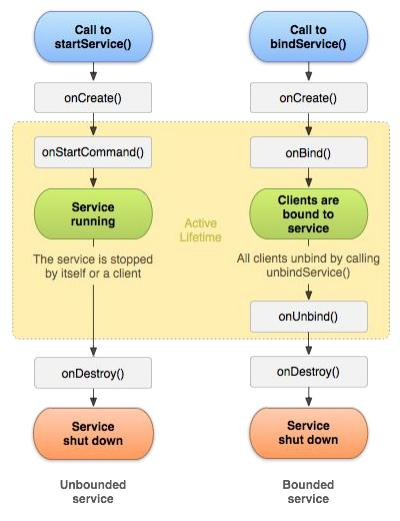
\includegraphics[width=0.4\linewidth]{images/service_lifecycle}
\caption{Service Lifecycle}
\label{fig:servicelifecycle}
\end{figure}




\section{Design Patterns}
\subsection{Multitier Architecture}
Unterteilung in 3 Layer. (Larman hat sogar 6 Schichten) Jeder Layer darf nur auf den direkt unter ihm liegenden zugreifen. Jeder Layer darf keine Abhängigkeiten zu den oberen Layer haben.
\begin{enumerate}
	\item Presentation: Zuständig für die Darstellung und Interaktion mit dem Benutzer
	\item Domain: Busineslogik und Domainklassen ohne UI Funktionalität
	\item Data: Implementiert die Speicherung der Daten
\end{enumerate}


\subsection{MVC: Model View Controller}
MVC ist ein Pattern für die Organisation des Presentation Layers.
\begin{description}
	\item[Model] Beinhaltet die Daten (bei Android die Activit)
	\item[View] liest die Daten des Modells und zeigt diese an
	\item[Controller] enthält Events der View und manipuliert das Model
\end{description}

\begin{figure}[h]
\centering
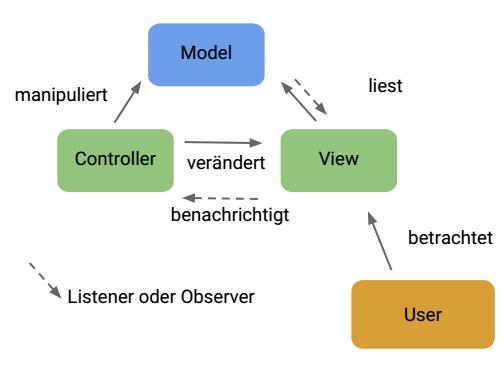
\includegraphics[width=0.7\linewidth]{images/mvc}
\caption{MVC: Model View Controller}
\label{fig:mvc}
\end{figure}



\subsection{Observer Pattern}
Da keine Zyklen zwischen den Layern erlaubt sind, ist der Einsatz des Observer Pattern notwendig. Damit Triggert das Datenmodell ein Update z.B. der angezeigten Liste.

\begin{quote}
Definiere eine 1-zu-n-Abhängigkeit zwischen Objekten, so dass die Änderung des 
Zustands eines Objekts dazu führt, dass alle abhängigen Objekte benachrichtigt und 
automatisch aktualisiert werden.
\end{quote}

Es gibt zwei Rollen:
\begin{description}
	\item[Subject / Observable] Subject welches beobachtet wird (z.B Model). In Java existiert bereits die abstrakte Klasse Observable
	\item[Observer] Observer welcher beobachtet (z.B View). In Java existiert bereits das Interface Observer
\end{description}

\begin{enumerate}
	\item Observer meldet sich beim Subject an, damit das Subject den Observer doch bitt informiert, sobald etwas geschehen ist
	\item Sobald der Observer benachrichtigt wird, holt er sich vom Subject den aktuellen Zustand. 
	\item Observer kennt Subject ziemlich gut, aber das Subject muss nichts über den konkreten Observer wissen.
\end{enumerate}

\begin{lstlisting}
public class Stock extends Observable {
	private String name;
	private double price;
	private Date date;
	
	// Konstruktor, Getter
	
	private void setNewRandomPrice() {
		date = new Date();
		price += new Random().nextDouble() - 0.49;
		setChanged();
		notifyObservers();
	}
}
\end{lstlisting}

\begin{lstlisting}
public class StocksAdapter extends RecyclerView.Adapter<...> implements Observer {
	private ArrayList<Stock> dataset;
	public StocksAdapter(ArrayList<Stock> stocks) {
		dataset = stocks;
		for (Stock stock : stocks) {
			stock.addObserver(this);
		}
	}
	
	@Override
	public void update(Observable observable, Object data) {
		int position = dataset.indexOf(observable);
		notifyItemChanged(position);
	}
}
\end{lstlisting}


\begin{figure}[h]
	\centering
	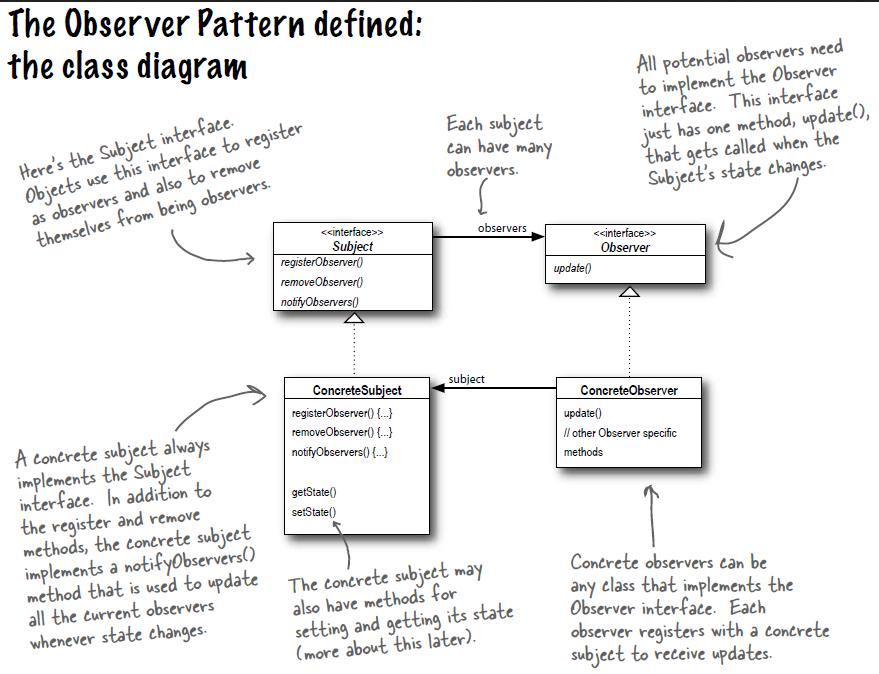
\includegraphics[width=0.8\linewidth]{images/observer}
	\caption{Observer Pattern UML}
	\label{fig:observer}
\end{figure}

\section{Sensoren}
Die meisten Mobiltelefone verfügen über diverse Sensoren, die jedoch von Gerät zu Gerät unterschiedlich sein können. Für die Arbeit mit Sensoren benötigt man einen \lstinline[]|SensorManager| (Einstiegspunkt für die verfügbaren Sensoren), \lstinline[]|Sensor| (Representant für einen konkreten Sensor), \lstinline[]|SensorEventListener| (Registrierung für Updates von Sensordaten) und \lstinline[]|SensorEvent| (Sensordaten auslesen)
\begin{lstlisting}[caption=Android Testing Erweiterung im build.gradle]
public class MainActivity extends AppCompatActivity implements SensorEventListener {
	private TextView textView;
	private SensorManager sensorManager;
	private Sensor lightSensor;
	
	@Override
	protected void onCreate(Bundle savedInstanceState) {
		...
		textView = (TextView) findViewById(R.id.textView);
		sensorManager = (SensorManager) getSystemService(Context.SENSOR_SERVICE);
		lightSensor = sensorManager.getSensorList(Sensor.TYPE_LIGHT).get(0);
	}
	
	@Override
	protected void onResume() {
		super.onResume();
		sensorManager.registerListener(this, lightSensor, SensorManager.SENSOR_DELAY_NORMAL);
	}
	
	@Override
	protected void onPause() {
		super.onPause();
		sensorManager.unregisterListener(this);
	}
	
	@Override
	public void onSensorChanged(SensorEvent event) {
		textView.setText(String.format("Helligkeit: %.0f", event.values[0]));
	}
}
\end{lstlisting}

\section{Dependency Injection}
Die meisten Klassen haben Abhängigkeiten zu anderen Klassen. Abhängigkeiten sollten wenn möglich als Interface über den Konstruktor übergeben werden. Unter Android verwendet man dafür am einfachsten das Framework \lstinline[]|Dagger2|.

\begin{lstlisting}[caption=Dagger2 Dependency Injection]
@Module
public class LibraryServiceModule {
	@Provides
	@Singleton
	public LibraryService getLibraryService() {
		return new LibraryService();
	}
}
@Singleton
@Component(modules = {LibraryServiceModule.class})
public interface GadgeothekComponent {
	void inject(GadgeothekActivity activity);
}

public class Application extends android.app.Application {
	GadgeothekComponent component;
	public void onCreate() {
		component = DaggerGadgeothekComponent.builder().build();
	}
	public GadgeothekComponent getComponent() {  
		return component;
	}
}

public class GadgeothekActivity extends AppCompatActivity {
	@Inject
	LibraryService libraryService;
	@Override
	protected void onCreate(Bundle savedInstanceState) {
		...
		((Application) getApplication()).getComponent().inject(this); 
	}
\end{lstlisting}

\subsection{View Injection}
Für die View Injection sollte das Framework \lstinline[]|Butter Knife| verwendet werden, welches die Arbeit mit GUI Elemente enorm vereinfacht.
\begin{lstlisting}[caption=View Injection mit Butter Knife]
class ExampleActivity extends Activity {
	@Bind(R.id.username) EditText username;
	@Bind(R.id.password) EditText password;
	@BindString(R.string.login_error) 
	String loginErrorMessage;

	@OnClick(R.id.submit) 
	void submit() {
		...
	}
	
	@Override 
	public void onCreate(Bundle savedInstanceState) {
		super.onCreate(savedInstanceState);
		setContentView(R.layout.simple_activity);
		ButterKnife.bind(this);
		...
	}
}
\end{lstlisting}


\subsection{Data Binding}
Data Binding wird von Android standardmässig unterstützt. Der grosse Vorteil ist, dass die Daten automatisch auf der View aktualisiert werden. Man muss aber aufpassen dass nicht zu viel Logik ins XML wandert. Dies würde dann auch dazu führen, dass die App schwieriger zu debuggen ist.
\begin{lstlisting}[caption=Data Binding]
// Model
public class User {
//
	public ObservableField<String> firstName = new ObservableField<>();
	public ObservableField<String> lastName  = new ObservableField<>()
		
	public TextWatcher lastNameWatcher = new TextWatcher() {
		
		@Override
		public void onTextChanged(CharSequence s, int start, int before, int count) {
			if (!Objects.equals(lastName.get(), s.toString())) {
				lastName.set(s.toString());
			}
		}	
	}
}

// Activity
public class MainActivity extends AppCompatActivity {
	@Override
	protected void onCreate(Bundle savedInstanceState) {
		super.onCreate(savedInstanceState);
		ActivityMainBinding binding = 
		DataBindingUtil.setContentView(this, R.layout.activity_main);
		User user = new User("Mirko", "Stocker");
		binding.setUser(user);
	}
}
\end{lstlisting}

\begin{lstlisting}[caption=Data Binding XML, language=XML]
<layout xmlns:android="http://schemas.android.com/apk/res/android">

	<data >
		<variable name="user" type="ch.hsr.mge.databindingdemo.User"/>
	</data>
	
	<RelativeLayout
		... >
		<TextView 
			android:text="@{user.firstName}"
			android:text="@{String.valueOf(index + 1)}"
			android:visibility="@{age < 13 ? View.GONE : View.VISIBLE}"
			android:transitionName='@{"image_" + id}'
			/>
		
		<Button
			android:text="Save"
			android:onClick="@{controller.onButtonSaveClicked}"/>
			
		<EditText
			android:text="@{user.lastName}"
			android:addTextChangedListener="@{user.lastNameWatcher}" />
	</RelativeLayout>
</layout>
\end{lstlisting}


\section{Android Selbststudium}
\subsection{Unit Testing}
Bei der Entwicklung mit Android werden die Java typischen JUnit 4 Tests eingesetzt. Man unterscheidet dabei zwischen zwei Varianten von Unit Tests:

\paragraph{Local Unit Tests}
Lokale Unit Tests sind unter \lstinline|module-name/src/test/java/| zu finden und werden auf lokalen JVM ausgeführt. Die Tests haben keinen Zugriff auf die Android Framework API's. Die Tests werden mit dem Mocking Framework Mockito\footnote{\url{https://github.com/mockito/mockito}} vom Rest des Systems isoliert und die Abhängikeiten mit Mock Objekten ersetzt.

\paragraph{Instrumental Tests / User Interface Tests}
Mit User Interface Tests versucht man herauszufinden ob die Obefläche der App einfach zu verstehen ist. Dazu kann man entweder menschliche Tester angagieren oder eine Test App in Android Studio schreiben. Instrumental Tests sind unter \lstinline|module-name/src/androidTest/java/| zu finden und müssen auf einem Android Gerät ausgeführt werden. Möglich ist auch ein Android Emulator.

\begin{figure}[h]
\centering
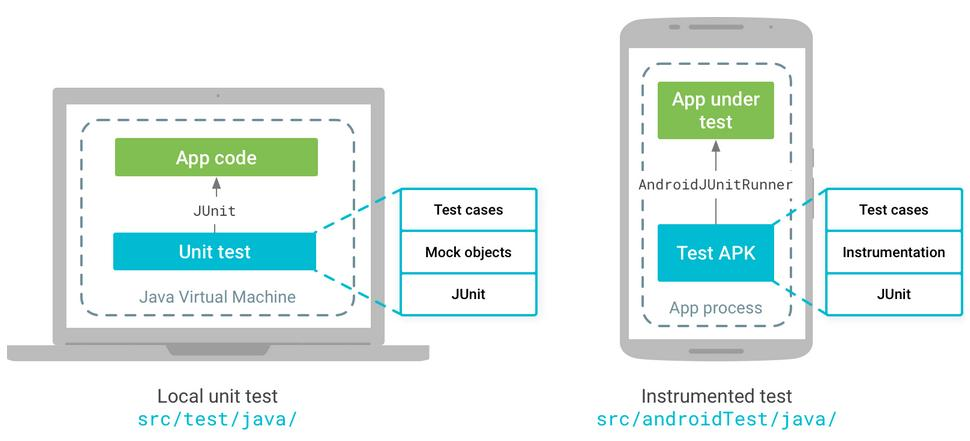
\includegraphics[width=0.7\linewidth]{images/unit_tests}
\caption{Unit Test Varianten unter Android}
\label{fig:unittests}
\end{figure}

\subsection{Integration Tests}

\paragraph{Components within your App}
Diese Art von Tests überprüft ob die App wie erwartet auf Benutzereingaben reagiert. Dies kann programtechnisch z.B mit dem Framework Espresso\footnote{\url{https://developer.android.com/topic/libraries/testing-support-library/index.html\#Espresso}} umgesetzt werden.

\paragraph{Cross-app Components}
Diese Art von Tests überprüfen das korrekte Verhalten von mehreren Apps während deren Kommunikation miteinander. z.B Mit dem Framework UI Automator\footnote{\url{https://developer.android.com/topic/libraries/testing-support-library/index.html\#UIAutomator}} können solche Szenarien erstellt werden. 

\subsection{Testumgebung einrichten}
\begin{enumerate}
	\item Tools > Android > SDK Manager
	\item Android Support Repository selektieren
	\item Apply
	\item im build.gradle folgendes hinzufügen
	\begin{lstlisting}[caption=Android Testing Erweiterung im build.gradle]
dependencies {
	androidTestCompile 'com.android.support:support-annotations:24.0.0'
	androidTestCompile 'com.android.support.test:runner:0.5'
	androidTestCompile 'com.android.support.test:rules:0.5'
	// Optional -- Hamcrest library
	androidTestCompile 'org.hamcrest:hamcrest-library:1.3'
	// Optional -- UI testing with Espresso
	androidTestCompile 'com.android.support.test.espresso:espresso-core:2.2.2'
	// Optional -- UI testing with UI Automator
	androidTestCompile 'com.android.support.test.uiautomator:uiautomator-v18:2.1.2'
}
	\end{lstlisting}
\end{enumerate}

\subsection{Firebase Test Lab}
Das Firebase Test Lab ermöglicht es, eine App auf unterschiedlichen Geräten zu testen, ohne diese Geräte wirklich physisch zur Hand zu haben. Die Geräte können von Google gemietet werden und die Tests laufen in einem externen Datencenter ab. \footnote{\url{https://firebase.google.com/docs/test-lab/}}

\subsection{JUnit 4}
\begin{lstlisting}[caption=Andorid JUnit 4 Test Beispiel]
@RunWith(AndroidJUnit4.class)
@LargeTest
public class MainActivityInstrumentationTest {

@Rule
public ActivityTestRule mActivityRule = new ActivityTestRule<>(MainActivity.class);

@Test
public void sayHello(){
onView(withText("Say hello!")).perform(click());

onView(withId(R.id.textView)).check(matches(withText("Hello, World!")));
}
}
\end{lstlisting}

\subsubsection{Test Suite}
Um mehrere Tests zu Gruppieren und gleichzeitig auszufügen, werden Test Suiten eingesetzt. Nach Konvention werden Testsuiten immer in einem Package mit dem .suite Suffix abgelegt (\lstinline|com.example.android.testing.mysuite.suite|)
\begin{lstlisting}[caption=Andorid JUnit 4 Test Suite]
// Runs all unit tests.
@RunWith(Suite.class)
@Suite.SuiteClasses({FirstTest.class,
SecondTest.class})
public class UnitTestSuite {}
\end{lstlisting}

\subsubsection{Annotations}
\begin{description}
	\item[@Before] Wird vor jedem Test ausgeführt. Wird für Setup Operationen verwendet.
	\item[@After] Wird nach jedem Test ausgeführt. Wird für tear-down Operationen verwendet.
	\item[@Test] Markiert eine Test Methode
	\item[@Rule] %TODO Whats That?
	\item[@BeforeClass] Hiermit werden statische Methoden annotiert, die z.B eine Verbindung zur Datenbank aufbauen.
	\item[@AfterClass] Hiermit werden statische Methoden annotiert, die z.B die Ressourcen die in @BeforeClass alloziert wurden, wieder freigibt. 
	\item[@Test(timeout=)] Gibt die maximale Zeit in ms an, wie lange der Test dauern darf. Danach schlägt der Test fehl.
\end{description}

\section{WPF: Windows Presentation Foundation}
WPF ist bestandteil des .NET Frameworks und wird für die Programmierung von Desktop Apps verwendet. Als Programmiersprache kommt C\# zum Einsatz.

\subsection{Logical und Visual Tree}
\begin{description}
	\item[Logical Tree] Eigene XAML Elemente
	\item[Visual Tree] Von WPF Dargestellte UI Elemente und Dekorationen
\end{description}

\begin{figure}[h]
\centering
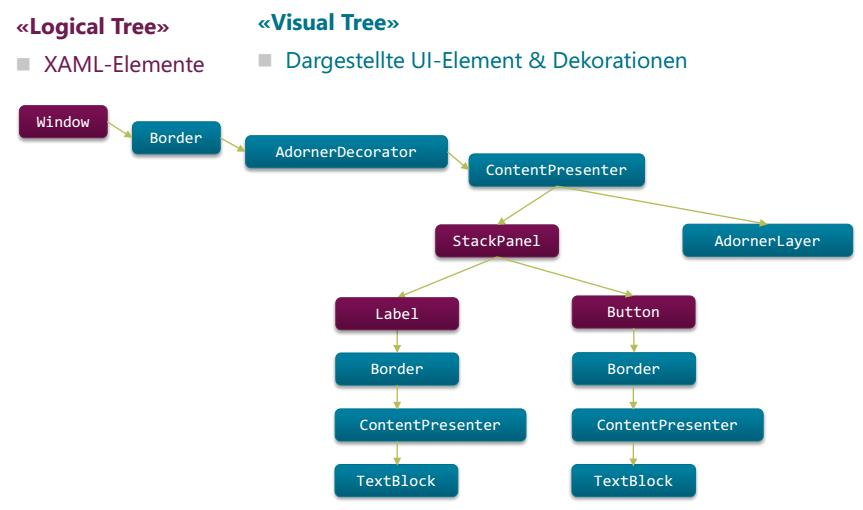
\includegraphics[width=0.7\linewidth]{images/wpf_overview}
\caption{WPF Klassen Übersicht}
\label{fig:wpfoverview}
\end{figure}

\subsection{XAML: Extensible Application Markup Language}
XAML ist eine XML-basierende Beschreibungssprache für WPF GUI's. Das XAML Markup wird zur Laufzeit mit dem Source Code zu einem Objekt verschmolzen und auf der CLR ausgeführt. Aus diesem Grund könnte man alle GUI Elemente auch einfach in C\# deklarieren. Die XAML Definiton ist gegenüber C\# Deklaration leichtgewichtiger und sollte deshalb vorgezogen werden. In XAML gibt es einen default XML Namespace mit dem Namen \lstinline|x:[Key]|.

XAML wird also in C\#-Objekte umgewandelt; zum Teil können damit mehr Objekte erstellt werden, als tatsächlich im XML deklariert sind (Z.B. Border-Objekte).

Attribute können im XAML als Child-Tags definiert werden.

\lstinline[language=xml]|<Button><Button.Content>asdf</.></.>| ist daher das Gleiche wie \lstinline[language=xml]|<Button Content="asdf"/>|.

\subsection{CLR: Common Language Runtime}
Die \gls{clr} umfasst mehrere Funtionen wie z.B Just In Time Compilation für die Übersetzung von Intermediate Language Code in Maschinencode. Man versteht unter dem \gls{clr} ein sprachunabhängiges, abstrahiertes Betriebssystem. Es ist verantwortlich für das Memory Management, Garbage Collection, Debugging und Threading.

\subsection{Device Independent Pixels}
Wie auch bei Android wird auch bei WPF mit Device Independent Pixels gearbeitet. 

\subsection{NuGet}
Nuget ist ein Package Management System für Visual Studio Projekte. Es bietet Packages wie z.B EntityFramework (O/R Mapper), Json.NET, Bootstrap CSS, jQuery, log4net, Xamarin.Forms, RestSharp, System.Data.SQLite etc. NuGet Packete werden über Project > Manage NuGetPackages hinzugefügt.


\section{C\# Grundlagen}
\subsection{Properties}
\begin{lstlisting}[caption=C\# Properties]
public class Person
{
	// backing field for property LastName
	private string _lastName;

	// property using explicit getter and setter
	public string LastName {
		get { return _lastName; }
		set { _lastName = value; }
	}
	
	// auto-implemented property (with automatically allocated backing field)
	public string FirstName { get; set; }

	// getter/setter body can be anything (e.g. Read-Only computed property)
	public string FullName {
		get {
			var fullName = LastName + " " + FirstName
			return fullName;
		}
	}

	// Lambda-syntax (C# >=6.0)
	public string FullNameFirstLast => FirstName + " " + LastName;
}
\end{lstlisting}


\subsection{Delegates}
Ein Delegate ist ein Funktionszeiger auf eine Funktion. Das Delegate definiert ähnlich einem Interface die Signatur der Funktion. (Methodensignatur) \lstinline[]|Action| und \lstinline[]|Func| (Lamda) sind vordefinierte Delegates
\begin{lstlisting}[caption=C\# Delegates]
namespace DelegateExample
{
	class Program {
		delegate int Calculation(int a, int b);
		static void Main(string[] args) {
			int x = 2;
			int y = 3;
			Calculation add = delegate(int a, int b) { return a + b; };
			int answer = add(x, y);
			System.Console.WriteLine(answer); // output: 5
		}
	}
}
\end{lstlisting}

\subsubsection{Vordefinierte Delegates}
\paragraph{Action} \hfill  \\
\begin{lstlisting}
void Action()
void Action<T>(T t)
void Action<T,U>(T t, U u)
// etc.
\end{lstlisting}

\paragraph{Func} \hfill \\
\begin{lstlisting}
TResult Func<TResult>()
TResult Func<T, TResult>(T t)
TResult Func<T, U, TResult>(T t, U u)
// etc.
// Beispiel:
Func<int,int> func1 = delegate(int x) { return x+1; }
\end{lstlisting}

\subsection{Lamdas}
\begin{lstlisting}[caption=C\# Lamdas]
static void Main(string[] args) {
	int x = 2;
	int y = 3;
	Func<int, int, int> add = (a, b) => a + b;
	int answer = add(x, y);
	System.Console.WriteLine(answer); // output: 5
	
	// Use implicitly typed lambda expression.
	Func<int, int> func3 = x => x + 1;
	// Use lambda expression with statement body.
	Func<int, int> func4 = x => { return x + 1; };
	// Use formal parameters with expression body.
	Func<int, int> func5 = (int x) => x + 1;
	// Use parameters with a statement body.
	Func<int, int> func6 = (int x) => { return x + 1; };
	// Use multiple parameters.
	Func<int, int, int> func7 = (x, y) => x * y;
	// Use no parameters in a lambda expression.
	Action func8 = () => Console.WriteLine();
}
\end{lstlisting}

\subsection{Events}
Events folgen dem Publish/Subscribe Mechanismus. Dass heisst es gibt Objekte, die Events triggern (Publish) und andere Objekte die auf diese Objekte hören (Subscribe.) 
\begin{lstlisting}[caption=C\# Events]
public class Person {

	// the event declaration
	public event EventHandler<PersonNameChangedEventArgs> NameChanged;

	// the method which encapsulates raising the event
	protected virtual void OnNameChanged(PersonNameChangedEventArgs e) {
		if (NameChanged != null) {
			NameChanged(this, e);
		}
	}
}
\end{lstlisting}

\subsection{EventHandler}
\begin{lstlisting}[caption=C\# Event Handler]
public delegate void EventHandler<TEventArgs>(object sender, TEventArgs e)
	where TEventArgs : System.EventArgs;
\end{lstlisting}

\subsection{Extension Methods}
Extension Methods sind statische Methoden die bestehendne Klassen hinzugefügt werden können. 
\begin{lstlisting}[caption=C\# Extension Methods]
public static class FileExtensions {
	public static string ToFileSize(this long size) {
		var units = new[] { "B", "KB", "MB", "GB", "TB" };
		var pow = 0;
		while (size >= 1024 && pow < units.Length) {
			size /= 1024;
			pow++;
		}
		return $"{size} {units[pow]}";
	}
}
\end{lstlisting}

\subsection{Formatierete Strings}
\begin{lstlisting}[caption=C\# Events]
string.Format("{0} changed name to {1}", a.OldName, a.NewName);
// Oder kuerzer:
$"{a.OldName} changed name to {a.NewName}"
\end{lstlisting}

\subsection{LINQ}
LINQ ist eine Sammlung von Extension Methods zur Abfrage und Manipulation von Daten. (Collections, SQL, XML)
\begin{lstlisting}[caption=LINQ]
var students;

// Query Syntax
var q = from s in students
	where s.Grade < 4m
	select s.FirstName + " " + s.LastName;

// Method Syntax
var q = students
	.Where(s => s.Grade < 4m)
	.Select(s => s.FirstName + " " + s.LastName);
	
foreach (var i in q) {
	Console.WriteLine(i);
}
\end{lstlisting}

\section{Controls}
\subsection{Properties}
Die WPF Controls verfügen über eine vielzahl von Eigenschaften:
\paragraph{Grössenangaben}
Mit \lstinline|Width| und \lstinline|Height| können die Grössen standardmässig mit Device Independet Pixels angegeben werden. (1px = 1/96 Zoll) Es kann auch \lstinline|auto| verwendet werden

\paragraph{Ausrichtung}
Mit \lstinline|HorizontalAlignment| und \lstinline|VerticalAlignment| kann die Ausrichtung definiert werden. \lstinline|Stretch| wird die verfügbare Höhe/Breite verwendet. 

\paragraph{Clipping}
Sollen Child Controls beim Rand des Parent abgeschnitten muss dies mit \lstinline|ClipToBounds="True"| angegeben werden. (default false)

\paragraph{Rahmen und Abstände} 
Mit \lstinline|Margin|, \lstinline|Padding|, \lstinline|BorderThickness| und \lstinline|CornerRadius| können die Ränder und Abstände definiert werden.
\begin{lstlisting}[caption=Borders, language=XML]
<Button Width="100"
	Height="60"
	BorderThickness="4"
	Margin="10,10,40,40" // (l, t, r, b)
	Padding="30,20"  // (l+r, t+b)
	Content="Element" 
	CornerRadius="tl" /> // top left (tl, tr, br, bl)
\end{lstlisting}

\paragraph{Sichtbarkeiten}
Mit \lstinline|IsEnabled| (interaktion möglich?), \lstinline|SnapsToDevicePixels|(Pixel Rendering) und \lstinline|Visibility| (collapse, hidden, visible) kann die Sichtbarkeit verändert werden.  

\paragraph{Farben und Schriften}
Mit \lstinline|Background|, \lstinline|BorderBrush|, \lstinline|Foreground| (Schriftfarbe), \lstinline|FontFamily|, \lstinline|FontSize|, \lstinline|FontStretch|, \lstinline|FontStyle| (Normal, Italic, Oblique), \lstinline|FontWeight| (ExtraBold, Bold, SemiBold, Normal, Light, ExtraLight) können die Farben und Schriften festgelegt werden. Zusätzlich gibt es 6 verschiedenen Pinseltypen, wie z.B eine Hintergrundfarbe dargestellt werden soll. (SolidColorBrush, LinearGradientBrush, ImageBrush, etc.)

%TODO Update Controls exmaples from appendix slides

\subsection{Container}
Man unterscheidet zwischen Container Controls mit und ohne Layout.

\subsubsection{StackPanel}
Das StackPanel ordnet alle Child Components der Reihe nach in eine Richtung an. Es gehört zu den Container mit Layout. Das Stack Panel füll den verfügbaren leeren Platz nicht aus. (d.h nich für Responsives Design geeignet)
\begin{figure}[h]
\centering
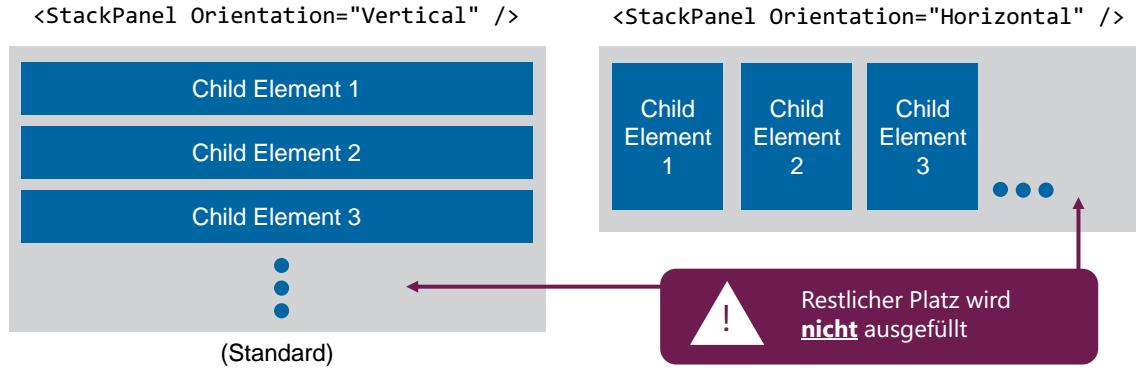
\includegraphics[width=0.5\linewidth]{images/stackpanel}
\caption{StackPanel}
\label{fig:stackpanel}
\end{figure}


\subsubsection{WrapPanel}
Das WrapPanel bricht im Gegensatz zum Stackpanel beim Zeilen-, Spaltenumbruch um. Ansonsten ist es gleich wie das StackPanel. Es wird selten gebraucht.

\subsubsection{DockPanel}
Alle Child Controls werden an einer Seite oder dem Zentrum angedockt. Das DockPanel füllt standardmässig mit dem letztem Child Control den verfügbaren Platz aus.
\begin{lstlisting}[caption=Dockpanel, language=XML]
<DockPanel>
	<TextBlock Test="" DockPanel.Dock="Left" />
	<TextBlock Test="" DockPanel.Dock="Right" />
	<TextBlock Test="" DockPanel.Dock="Top" />
	<TextBlock Test="" DockPanel.Dock="Bottom" />
	<TextBlock Test="Center" />
</DockPanel>
\end{lstlisting}
\begin{figure}[h]
\centering
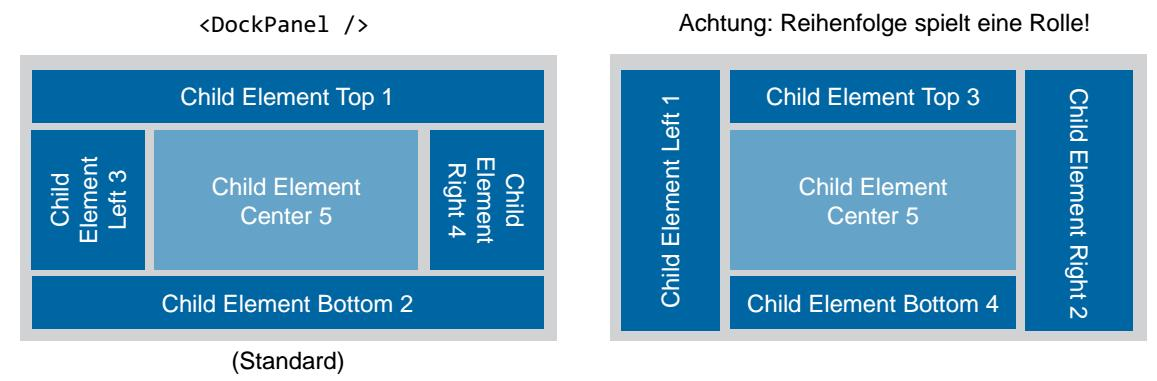
\includegraphics[width=0.5\linewidth]{images/dockpanel}
\caption{Dockpanel}
\label{fig:dockpanel}
\end{figure}

\subsubsection{Grid}
Die Child Controls werden den Zellen einer manuell definierten Tabelle zugeordnet. Jeder Spalte/Zeile können breiten und höhen hinzugefügt werden. 
\begin{itemize}
	\item Ganzzahl: Fixe Angabe
	\item Auto: Automatisch aus verfügbarem Platz und Inhalt
	\item *: Nutzt ganze Breite/Höhe entsprechend dem verfügbaren Rest (proportional aufgeteilt, falls mehrere)
	\item 2*: Gewichtete Angabe
\end{itemize}
\begin{lstlisting}[caption=Grid, language=XML]
<Grid>
	<Grid.ColumnDefinitions>
		<ColumnDefinition Width="50"></ColumnDefinition>
		<ColumnDefinition Width="Auto" MinWidth="40"></ColumnDefinition>
		<ColumnDefinition></ColumnDefinition>
	</Grid.ColumnDefinitions>
	<Grid.RowDefinitions>
		<RowDefinition Height="50" MaxHeight="70"></RowDefinition>
		<RowDefinition Height="*"></RowDefinition>
		<RowDefinition ></RowDefinition>
	</Grid.RowDefinitions>
	
	<!-- Plaziere Button oben links ueber 3 Spalten  und 3 Reihen ->
	<Button Grid.Column="0" Grid.Row="0" Grid.RowSpan="3" Grid.ColumnSpan="3" />
</Grid>
\end{lstlisting}

\subsubsection{Canvas}
Das Canvas hat im Gegensatz zu den vorgehenden Container keine Layout Logik. In Canvas können Geometrische Elemente (Shapes) hineingezeichnet werden.


\subsection{ViewBox}
Eine ViewBox skaliert das Child Element auf die Grösse, die über die \lstinline|Stretch|-Property (None, Fill, Uniform, UniformToFill) übergeben wird.

\subsection{Image}
Das Image Controll zeigt ein Bild an und skaliert dieses auf die selbe Weise, wie es die ViewBox mit den Child Controls macht.

\subsection{Border}
Das Border Control zeichnet einen Rahmen um das Child Control. Es kann mit Panels kombiniert werden.

\subsection{Dialogfenster}
Dialogfenster bieten ein modales Fenster mit einer Auswahl.
\begin{lstlisting}[caption=Dialog, language=XML]
// Schliesst automatisch, kein Event Handler noetig
<Button Content="Abbrechen" IsCancel="true" />
<Button Name="OkButton" Content="OK" IsDefault="true" Click="OkButton_OnClick" />
\end{lstlisting}

\begin{lstlisting}[caption=Dialog]
private void OkButton_OnClick(object sender, RoutedEventArgs e) {
	SelectedCustomer = "Max Muster";
	DialogResult = true; // schliesst das Fenster!
}

private void OpenDialog_OnClick(object sender, RoutedEventArgs e) {
	var win = new DialogWindow();
	if (win.ShowDialog() != true) {
		Debug.WriteLine("Cancelled :-(");
		return;
	}

	Debug.WriteLine("OK :-)");
	var chosenCustomer = win.SelectedCustomer;
	...
}
\end{lstlisting}

\section{Commands}
Command sind eine Alternative zu UI Events, wobei ein Befehl standartisiert ausgeführt werden soll. Commands ermöglichen die Wiederverwendung derselben Aktionen. Dazu sind folgende Schritte nötig:
\begin{enumerate}
	\item Defintions eines eigenen Commands als statische Instanz von RoutedUICommand in einer beliebigen Klasse
	\item Nutzung durch setzen des Command Attributes auf die statische Instanz
	\item CommandBinding-Element auf Ebene Window setzen
	\item Für Tastenkürzel: KeyBinding-Element auf Ebene Window setzen
	\item Via Command-(Event) Handler Code ausführen
\end{enumerate}
\begin{lstlisting}[caption=Commands]
// 1. Definition
public static RoutedUICommand MyCutCommand = new RoutedUICommand("Ausschneiden", "MyCut", typeof(WindowWithToolbar));

// 5. Implementation
private void MyCutCommand_Executed(object sender, ExecutedRoutedEventArgs e)
{
...
}
\end{lstlisting}

\begin{lstlisting}[caption=Commands, language=XML]
<!-- 2. local: ist der Namespace im XML. Verweis auf das aktuelle Projekt -->
<MenuItem Header="_Cut" InputGestureText="CTRL + X"
		Command="local:MyClass.MyCutCommand" />
	
<!-- 3. Binden an Command-(Event) Handler -->	
<Window.CommandBindings>
	<CommandBinding Command="local:WindowWithToolbar.MyCutCommand" Executed="MyCutCommand_Executed" />
</Window.CommandBindings>

<!-- 4. Shortcuts definieren -->
<Window.InputBindings>
	<KeyBinding Key="X" Modifiers="Control" Command="local:WindowWithToolbar.MyCutCommand" />
</Window.InputBindings>
\end{lstlisting}


\section{Resources}
Mit Ressourcen lassen sich Objekte (Pinsel, Styles oder Templates) zentral definieren und hinterlegen. Dies fördert die Wiederverwendbarkeit (Ein Mal definieren und N-Mal verwenden).

\begin{lstlisting}[caption=Resources, language=XML]
<!-- definition x: = Default XAML XML namespace -->
<!-- application scope -->
<Application.Resources>
	<SolidColorBrush x:Key ="MyButtonBackground" Color="#EEEEEE" />
</Application.Resources>

<!-- window scope -->
<Window.Resources>
<SolidColorBrush x:Key ="MyButtonBackground" Color="#EEEEEE" />
</Window.Resources>

<!-- use -->
<!-- fix after compilation -->
<Button Background="{StaticResource MyButtonBackground}" Content="Save" /> 
<!-- fetch every time -->
<Button Background="{DynamicResource MyButtonBackground}" Content="Save" /> 
\end{lstlisting}

\subsection{ResourceDictionary}
Resourcen werden in einem \lstinline|ResourceDictionary| gespeichert und über den Ressourcen-Namen (\lstinline|x:Key|) indexiert. Es gibt auf mehreren Ebenen ein Resource Dictionary. (Button.Resources, Window.Resources, Application.Resources). Der Key wird entlang dem logischen Baum von Unten nach Oben gesucht. 

\subsubsection{Eigene Resourcen}
Ein Resource Dictionary ist ein normales .xaml File.
\begin{lstlisting}[caption=Eigene Resource Dictionaries, language=XML]
<Application.Resources>

	<ResourceDictionary>
		
		<!-- include your base dictionaries, here -->
		<ResourceDictionary.MergedDictionaries>
			<ResourceDictionary Source="ExternalResourceDictionary.xaml"/>
		</ResourceDictionary.MergedDictionaries>
		
		<!-- now, access the externally defined resources -->
		<SolidColorBrush x:Key="ButtonBgBrush" Color="{StaticResource ThemeColor1}" />
		
	</ResourceDictionary>
	
</Application.Resources>
\end{lstlisting}

\subsection{System Resources}
Im Namespace \lstinline|System.Windows| hat man Zugriff auf verschiedenste statische Properties wie z.B \lstinline|SystemColors.WindowTextColor|, \lstinline|SystemFonts.MenuFontFamily| und \lstinline|SystemParameters.PrimaryScreenWidth| etc.


\subsection{Resourcen in C\#}
In C\# kann mittels \lstinline|FindResource()| auf eine Ressource zugegriffen werden. Die Methode liefert ein Objekt zurück, weshalb immer gecasted werden muss.
\begin{lstlisting}[caption=Resources in C\#]
var okText = (string)FindResource("OkText");
var bgBrush = FindResource("DarkBrush") as Brush; // Andere Moeglichkeit zu casten
\end{lstlisting}


\section{Styles und Templates}
Wie Resourcen werden Styles über einen Key identifiziert. Der Key kann aber auch weggelassen werden und stattdessen \lstinline|TargetType="Button"| verwenden. Damit gilt der Style für alle Controls des angegebenen Typs. Bei grösseren Projekten, werden oft eigenen Style Projekte erstellt, bei welchen die Farben, Grafiken, Styles und Controlls in separaten Folder geführt werden.
\begin{lstlisting}[caption=Styles, language=XML]
<Style x:Key="MyButtonStyle">
	<Setter Property="Button.Foreground" Value="#2672EC" />
	<Setter Property="Button.BorderBrush" Value="#2672EC" />
	<Setter Property="Button.BorderThickness" Value="2" />
	<Setter Property="Button.FontFamily" Value="Segoe UI" />
	<Setter Property="Button.FontSize" Value="13" />
	<Setter Property="Button.Padding" Value="10 2 10 2" />
	<Setter Property="Button.Margin" Value="2" />
	<Setter Property="Button.Background">
		<Setter.Value>
			<LinearGradientBrush StartPoint="0,0" EndPoint="0,1">
				<GradientStop Offset="0" Color="#dddddd" />
				<GradientStop Offset="0.5" Color="#F0F0F0" />
				<GradientStop Offset="1" Color="#dddddd" />
			</LinearGradientBrush>
		</Setter.Value>
	</Setter>
</Style>

<!-- extend styles -->
<Style x:Key="DangerButtonStyle" 
	TargetType="Button"
	BasedOn="{StaticResource MyButtonStyle}">
	<Setter Property="Background" Value="Red" />
</Style>


<!-- usage -_>
<StackPanel Orientation="Horizontal">
<Button Style="{StaticResource MyButtonStyle}" Content="Cancel" />
<Button Style="{StaticResource MyButtonStyle}" Content="Ok" />
<Button Style="{StaticResource MyButtonStyle}" Content="Save" />
</StackPanel>
\end{lstlisting}

\subsection{Template}
\begin{lstlisting}[caption=Eigene Resource Dictionaries, language=XML]
<Setter Property="Template">
	<Setter.Value>
		<ControlTemplate TargetType="Button">
			<Border BorderBrush="{TemplateBinding BorderBrush}"
				BorderThickness="{TemplateBinding BorderThickness}">
				<StackPanel Orientation="Horizontal" Background="{TemplateBinding Background}">
					<Grid Margin="4" >
						<Ellipse x:Name="ButtonEllipse" Fill="{TemplateBinding Foreground}" Height="16" Width="16" />
						<Label Foreground="{TemplateBinding Background}" HorizontalContentAlignment="Center">!</Label>
					</Grid>
					<ContentPresenter Content="{TemplateBinding Content}" Margin="0 0 10 0" VerticalAlignment="Center" />
				</StackPanel>
			</Border>
		</ControlTemplate>
	</Setter.Value>
</Setter>
\end{lstlisting}

\subsection{Style Trigger}
Mit Style Trigger kann der Style anhand unterschiedlicher UI Zustände angepasst werden.
\begin{lstlisting}[caption=Eigene Resource Dictionaries, language=XML]
<Style x:Key="MyButtonStyle" TargetType="Button">
	<Setter Property="Background" Value="White" />
	<Setter Property="Foreground" Value="Black" />
	<Setter Property="Cursor" Value="Hand" />
	<Style.Triggers>
		<Trigger Property="IsMouseOver" Value="True">
			<Setter Property="Background" Value="#2672EC" />
			<Setter Property="Foreground" Value="White" />
		</Trigger>
	</Style.Triggers>
</Style>
\end{lstlisting}

\section{Data Binding}
Fürs Databinding werden die Klassen \lstinline|BindingBase|, \lstinline|Binding| und \lstinline|MultiBinding| verwendet.
\subsection{Markup Extensions}
\begin{itemize}
\item {x:Type [Datentyp]} Liefert angegebenen [Datentyp]/Klasse
\item{x:Static [Pfad]} Bindet an Konstante, statische Property oder Field, sowie an Enums
\item{x:Null} Null-Wert
\item{StaticResource [Name]} Statische Bindung an Ressource (Vgl. letzter Block)
\item{DynamicResource [Name]} Dynamische Bindung an Ressource (Vgl. letzter Block)
\item{Binding ...} Data Binding Ausdruck
\item{RelativeSource...} Setzt die Data Binding Source auf eine relativen Bezug im Logical Tree
\item{TemplateBinding...} Bindet Wert an Eigenschaft des mittels Template dargestellten Controls
(Vgl. letzter Block)
\item {x:Reference...} Abkuerzung fuer {Binding ElementName=...}
\end{itemize}

\subsection{Attribut Syntax und Property Syntax}
\begin{lstlisting}[caption=Data Binding, language=XML]
// Attribute Syntax
<TextBox Text="{Binding ScaleX, ElementName=WpfLabelScale, StringFormat={}{0:0.0} }"/>

<Label Width="35" Content="{Binding Path=Saturation, Converter={StaticResource DoubleToString}}"/>

<ListBox Name="colorListBox" ItemsSource="{Binding}" ItemTemplate="{StaticResource ColorItemTemplate}" />

<!-- Translated Strings oder Templates  -->
<Label Content="{Binding Source={StaticResource NameLabelCaption}}" />
<ContentControl Content="{Binding Source={StaticResource MyFriends}}"
		ContentTemplate="{StaticResource DetailTemplate}"/>

// Property Syntax
<TextBox>
	<TextBox.Text>
		<Binding Path="Angle" ElementName="WpfLabelRotate" StringFormat="{}{0:0.0}" />
	</TextBox.Text>
</TextBox>
\end{lstlisting}


\subsection{DataContext}
Standardmässig ist keine Datenquelle für die Bindings gesetzt. Diese muss manuell gesetz werden.
\begin{itemize}
	\item DataContext (default)
	\item Source (für jedes Binding eine andere Quelle)
	\item RelativeSource
	\item ElementName
\end{itemize}

\begin{lstlisting}[caption=Data Binding]
public partial class MainWindow : Window {
	public PersonViewModel MyViewModel { get; set; }
	
	public MainWindow() {
		InitializeComponent();
		MyViewModel = new PersonViewModel();
		DataContext = this; 
		// DataContext = MyViewModel;
	}
}

<TextBlock Text="{Binding MyViewModel.FirstName}" />
<!-- ist das gleiche wie: -->
<TextBlock><TextBlock.Text><Binding Path="MyViewModel.FirstName" /></.></.>
\end{lstlisting}


\begin{lstlisting}[caption=Dynamisches Data Binding]
public partial class MainWindow : Window {
	public ObservableCollection<PersonViewModel> PersonList { get; set; }

	public MainWindow() {
		InitializeComponent();
		var list = ...;
		PersonList = new ObservableCollection<PersonViewModel>(list);
		DataContext = this;        
	}
}

<ListBox ItemsSource="{Binding PersonList}" >...</ListBox>
\end{lstlisting}


\subsection{Path}
Path ist die Standard Property eins Binding Ausdrucks, und kann deshalb auch weggelassen werden, sofern nur eine Property gesetzt wird. 

\subsection{Mode}
Der Mode definiert die Richtung der Datenbindung
\begin{itemize}
	\item OneTime: Einmalig
	\item OneWay: Lesend
	\item TwoWay: Lesend und schreibend
	\item OneWayToSOurce: Schreibend
\end{itemize}

\subsection{Value Converter}
Converter werden verwendet um zwischen zwei Typen zu konvertieren. (z.B boolean $\leftrightarrow$ Enum). WPF liefert standardmässig einige Converter. Es gibt auch die Klasse \lstinline|IMultiValueConverter| wobei dort der \lstinline|value| Parameter ein \lstinline|object|-Array ist.
\begin{lstlisting}[caption=Dynamisches Data Binding]
public sealed class BooleanToVisibilityConverter : IValueConverter {
	public object Convert(object value, Type targetType, object parameter, CultureInfo culture) {
		return value is bool && (bool)value == true ? Visibility.Visible : Visibility.Collapsed;
	}
	public object ConvertBack(object value, Type targetType, object parameter, CultureInfo culture) {
		return value as Visibility? == Visibility.Visible;
	}
}
\end{lstlisting}

Die Converter können entweder als Resource oder als statische Property in einer C\# Klasse (nicht empfohlen) verwendet werden.
\begin{lstlisting}[caption=Value Converter, language=XML]
Application.Resources>
	<local:BooleanToVisibilityConverter x:Key="MyVisibilityConverter" />
</Application.Resources>

<!-- usage -->
<Label Visibility="{Binding IsAvailable, Converter={StaticResource MyVisibilityConverter}}" />
\end{lstlisting}


\subsection{Property Changed Interface}
\begin{lstlisting}[caption=INotifyPropertyChanged]
public class Person : INotifyPropertyChanged {

	private string _firstName;
	public string FirstName {
		get { return _firstName; }
		set { SetProperty(ref _firstName, value, nameof(FirstName)); }
	}

	public event PropertyChangedEventHandler PropertyChanged;
	private bool SetProperty<T>(ref T field, T value, string propertyName)
		// value ist der uebergeben Wert des Setters (value Keyword)
		if (Equals(field, value)) {
			return false;
		}
		field = value;
		
		PropertyChanged?.Invoke(this, new PropertyChangedEventArgs(propertyName))

		return true;
	}
}
\end{lstlisting}

\subsubsection{Berechnete Propeties}
\begin{lstlisting}[caption=INotifyPropertyChanged fuer berechnete Properties]
// Publish
private string _firstName;
public string FirstName {
	get { return _firstName; }
	set { SetProperty(ref _firstName, value, nameof(FirstName), nameof(FullName)); }
}
private string _lastName;
public string LastName {
	get { return _firstName; }
	set { SetProperty(ref _lastName, value, nameof(LastName), nameof(FullName)); }
}
protected bool SetProperty<T>(ref T storage, T value, string name, params string[] otherNames) {
	if (Equals(storage, value)) {
		return false;
	}
	storage = value;
	OnPropertyChanged(name);
	foreach (var n in otherNames) {
		OnPropertyChanged(n);
	}
	return true;
}

// Subscribe
public partial class App {

	public MyClass MyObject {get; set; }

	MyObject.PropertyChanged += (sender, args) => {
		var propertyName = args.PropertyName;
		var newValue = sender.GetType().GetProperty(args.PropertyName).GetValue(sender);
	};

}
\end{lstlisting}


\section{Events}
In C\# rsp. WPF kann man sich auf zwei Arten für Events anmelden
\begin{lstlisting}[caption=]
// Variante 1: Fuer Event subscriben
public partial class : Application {
	public App() {
		this.Startup += (o, args) => { .. }
	}
}

// Variante 2: Vorderfinierter virtueller Event Handler ueberschreiben
public partial class App: Application {
	protected override void OnStartup(StartEventsArgs e) { .. }
}
\end{lstlisting}

\subsection{App Startup}

\begin{figure}[h]
\centering
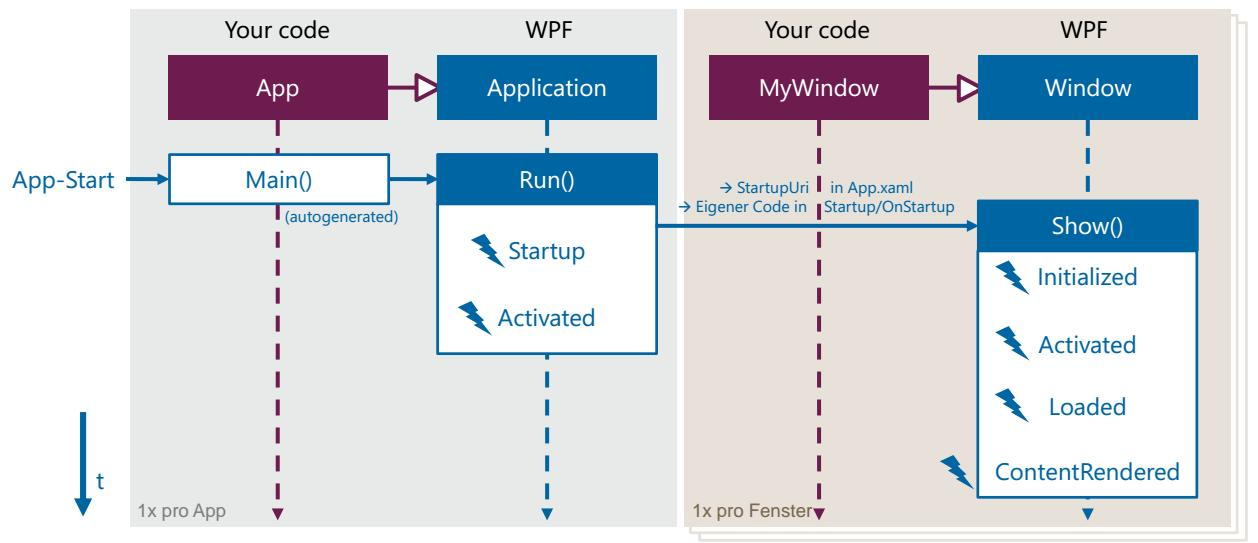
\includegraphics[width=0.7\linewidth]{images/app_startup}
\caption{App Startup}
\label{fig:appstartup}
\end{figure}

\subsection{Routet Events}
Routet Events sind interessante UI Ereignisse, auf die man reagieren kann. Routet Events können abgebrochen werden (Handled=true) und werden zuerst nach unten (Preview/Tunneling) und danach aufwärts (Bubbling) durch den Visual Tree gesendet.

\begin{description}
	\item[Preview] Reagieren auf den Event \lstinline|PreviewMyEvent| auf dem Weg zu dem Ziel Element nach unten (von Window aus)
	\item[Bubbling] Reagieren auf den Event \lstinline|MyEvent| auf dem Rückweg zurück zum Window
\end{description}

\begin{lstlisting}[caption=Routet Events]
<Buton Name="SaveButton" 
	PreviewMouseDown="SaveButton_OnPreviewMouseDown"
	MouseDown="SaveButton_OnMouseDown">Save</Button>
	
private void SaveButton_OnPreviewMouseDown(object sender, MouseButtonEventArgs e) {
	...
}
private void SaveButton_OnMouseDown(object sender, MouseButtonEventArgs e) {
	...
}
\end{lstlisting}

\begin{figure}[h]
\centering
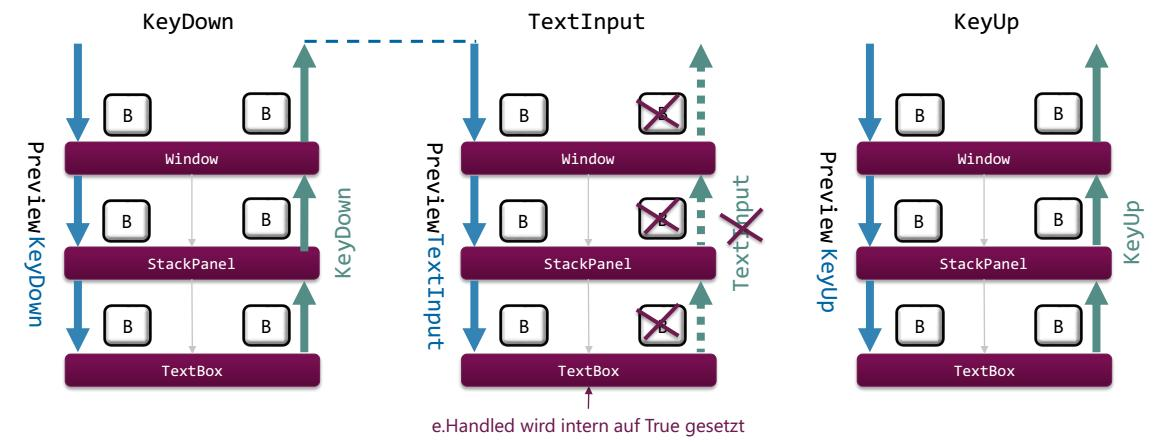
\includegraphics[width=0.7\linewidth]{images/routet_events}
\caption{Routet Events}
\label{fig:routetevents}
\end{figure}


\section{MVVM: Model View ViewModel}
\begin{figure}[h]
\centering
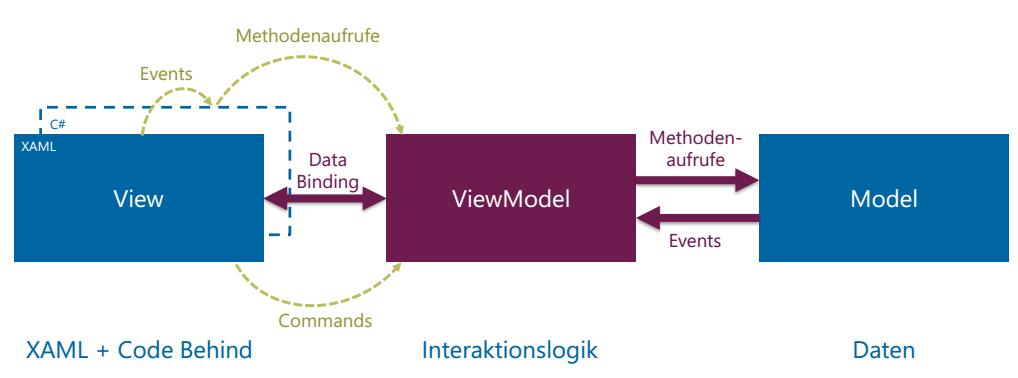
\includegraphics[width=0.7\linewidth]{images/mvvm}
\caption{MVVM: Klare Trennung zwischen Präsentation und Logik}
\label{fig:mvvm}
\end{figure}


\section{UI Testing}
Mit dem Framework Teststack White können Whitebox UI Tests erstellt werden. 
\begin{figure}[h]
\centering
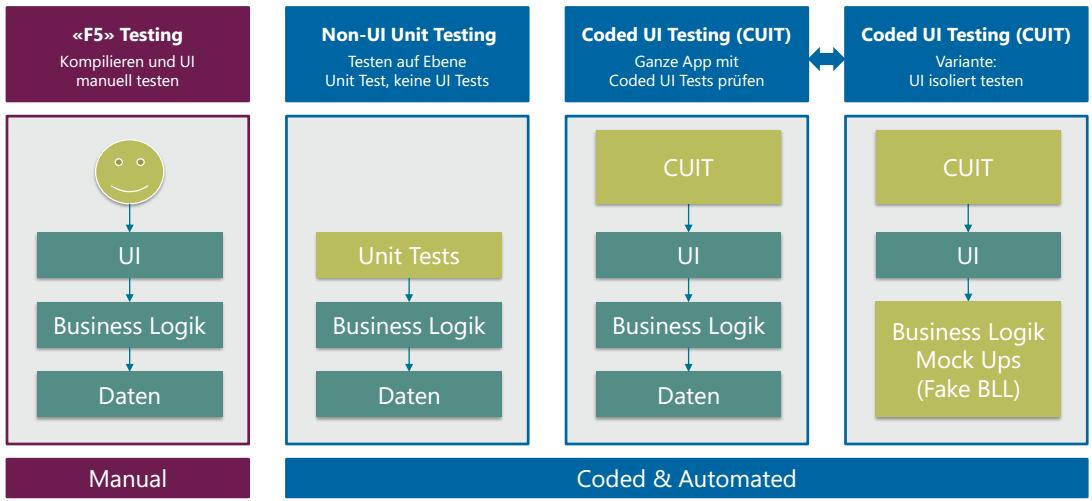
\includegraphics[width=0.7\linewidth]{images/ui_testing}
\caption{UI Testing}
\label{fig:uitesting}
\end{figure}





\appendix

% Code Listings
\lstlistoflistings

% List of figures
\listoffigures

% List of tables
\listoftables

% Bibliography
\bibliographystyle{plain} 
\bibliography{literatur}

\end{document}
